\documentclass[11pt,a4paper,oneside]{report}

% If you get an error that says you need to use LuaLaTex or XeLateX, you will need to change your compiler.  In Overleaf, this is done in the menu (upper left) which will open a drop down menu where you can change the default compiler to XeLaTeX.  This is necessary to support the special fonts.

\usepackage{svg}
\usepackage{float}
\usepackage{amsmath,amssymb}
\usepackage{parskip}
\usepackage{graphicx}
\usepackage{xcolor}
\usepackage[a4paper,margin=1in]{geometry}
\usepackage{longtable,booktabs,array}

\usepackage{titlesec}
\titleformat{\chapter}[display]
  {\sffamily\bfseries\huge}
  {\Large \chaptertitlename\ \thechapter}
  {2ex}
  {\titlerule
   \vspace{1ex}%
   \filright\MakeUppercase}
  [\vspace{1ex}%
\titlerule]
\titleformat{\section}{\normalfont\sffamily\Large\bfseries}{\thesection}{1em}{}
\titleformat{\subsection}{\normalfont\sffamily\large\bfseries}{\thesubsection}{1em}{}
\titleformat{\subsubsection}{\normalfont\sffamily\normalsize\bfseries}{\thesubsubsection}{1em}{}

\usepackage[style=numeric-comp, url=false]{biblatex}
\addbibresource{bibfile.bib}

\usepackage[no-math]{fontspec}
\usepackage{unicode-math}
\defaultfontfeatures{Ligatures=TeX,Numbers=Lining}
\usepackage[opentype]{sourceserifpro}
\setmainfont{Source Serif 4}[BoldFont={Source Serif 4 Semibold}]
\setsansfont{Source Sans 3}[BoldFont={Source Sans 3 Semibold}]
% \IfFontExistsTF{Cambria Math}{\setmathfont{Cambria Math}[Scale=1]}{\setmathfont{Asana Math}}

\usepackage{xeCJK}
\setCJKmainfont{Noto Sans CJK SC}
\setCJKsansfont{Noto Sans CJK SC}

\newcommand{\instructions}[1]{{\color{orange}\itshape #1}}
\renewcommand{\instructions}[1]{}

\usepackage{upquote}
\usepackage[allcolors=blue,colorlinks=true]{hyperref}
\usepackage{xurl}
\usepackage{microtype}
\usepackage{bookmark}
\usepackage{calc}
\usepackage{etoolbox}
\usepackage{longtable}
\urlstyle{same}

\begin{document}


% Author name (capitalized in its regular way)
\newcommand{\authorname}{Luyao Wang}

% Title (cannot exceed three lines)
\newcommand{\thetitle}{Exploring Machine Learning Application in League of Legends}

% Date of submission with normal capitalization. Use the format January 29, 2022.
\newcommand{\submissiondate}{April 6, 2024}

% Mentor: First Name Last Name (normal capitalization)
\newcommand{\mentor}{Pengzhan Guo}

% Academic Unit (no abbreviations)
\newcommand{\academicunit}{Division of Natural and Applied Sciences}

%%%%%%%%%%%%%%%%%%%%%%%%%%%%%%%%%%%%%%%%%%%%%%%%%%%%%%%%%%%%%%%%%%%%%%%%%%%%%%%%

%% DO NOT CHANGE DIRECTLY THE CONTENTS OF THE TITLE PAGE.
%% TO CUSTOMIZE THE TITLE PAGE CHANGE THE DEFINITIONS OF THE COMMANDS
%% \authorname, \thetitle, \submissiondate, \mentor, \academicunit

\begin{titlepage}

  \vspace*{\bigskipamount}

  \begin{center}
    {\sffamily\LARGE\bfseries\MakeUppercase\thetitle\par}

    \bigskip

    by

    \bigskip

    {\Large \authorname}

    \bigskip

    Signature Work Product, in partial fulfillment of the \\
    Duke Kunshan University Undergraduate Degree Program

    \bigskip

    \emph{\submissiondate}

    \bigskip

    Signature Work Program \\
    Duke Kunshan University

  \end{center}

  \vfill

  \textbf{\textsf{APPROVALS}}

  \bigskip\bigskip\bigskip
  \hrule

  Mentor: \mentor, \academicunit

  \bigskip\bigskip\bigskip
  \hrule

  Marcia B. France, Dean of Undergraduate Studies

\end{titlepage}

%%%%%%%%%%%%%%%%%%%%%%%%%%%%%%%%%%%%%%%%%%%%%%%%%%%%%%%%%%%%%%%%%%%%%%%%%%%%%%%%

% Front matter
\clearpage
\pagenumbering{roman}

%%%%%%%%%%%%%%%%%%%%%%%%%%%%%%%%%%%%%%%%%%%%%%%%%%%%%%%%%%%%%%%%%%%%%%%%%%%%%%%%

\setcounter{tocdepth}{0} % Only top-level units (chapters) should appear in the TOC
\tableofcontents

%%%%%%%%%%%%%%%%%%%%%%%%%%%%%%%%%%%%%%%%%%%%%%%%%%%%%%%%%%%%%%%%%%%%%%%%%%%%%%%%

\chapter*{Note}
\addcontentsline{toc}{chapter}{Note}

Source code of this project will be released in the \href{https://github.com/lywlywly/signature-work}{GitHub repo}.

\vspace{4\bigskipamount}


%%%%%%%%%%%%%%%%%%%%%%%%%%%%%%%%%%%%%%%%%%%%%%%%%%%%%%%%%%%%%%%%%%%%%%%%%%%%%%%%

\chapter*{Abstract}
\addcontentsline{toc}{chapter}{Abstract}

% Abstract in English

\instructions{Abstract (English): 150 -- 200 words. An abstract is a brief
  statement of the problem or the purpose of the research. It should indicate
  the theoretical work or experimental plan used, summarize principal findings
  of the research, and point out major conclusions. Appropriate safety
  information should be included when applicable. This should be the section
  you write last to be sure that it accurately reflects the content of the
  document.}

In the dynamic landscape of League of Legends, the integration of machine learning techniques has become increasingly valuable for strategic decision-making and accurate predictions. This is especially evident in the competitive landscape of LoL Esports, where in-game predictions play a prominent role in high-stakes tournaments like the Worlds and MSI. This project focuses on building pre-game and in-game prediction applications using the Riot API, LCU, and machine learning algorithms. The project involves data gathering from the Riot API and statistics websites, training machine learning models for pre-game and in-game predictions, and developing machine learning applications with Tauri and React, along with backend integration with the League Client. Word embedding techniques are employed to obtain champion and item vector embeddings and assess their compatibility. LSTM models are used for real-time in-game win rate prediction, while logistic regression is employed for the pre-game ban/pick phase prediction. By leveraging the Riot API, LCU, and machine learning techniques, this project aim to provide valuable predictions and insights to players, empowering them to make informed decisions and improve their performance on the Summoner's Rift.

\vspace{4\bigskipamount}

%%%%%%%%%%%%%%%%%%%%%%%%%%%%%%%%%%%%%%%%%%%%%%%%%%%%%%%%%%%%%%%%%%%%%%%%%%%%%%%%

\chapter*{Acknowledgements}
\label{acknowledgements}
\addcontentsline{toc}{chapter}{Acknowledgements}

\instructions{Individuals and organizations who helped with the research project
  and provided financing are thanked in a paragraph of the thesis. Do not
  include individual titles in the acknowledgments. However, it is
  appropriate to state grant numbers and sponsors. Examples would like
  SELF, SRS, SW Grants, etc.}

I would like to acknowledge the inspiration from \href{https://github.com/Java-S12138}{Java-S12138}, a GitHub user who developed the open-source application called Record \cite{record}. This application served as the foundation for the pre-game prediction application for League of Legends I built in this project. My interest in League of Legends prediction and building related applications was sparked by \href{https://www.bilibili.com/video/BV1nU4y1D7FQ/}{a video by him}. Through this video, I discovered the immense programmability and possibilities within the League of Legends ecosystem.

% Additionally, another open-source project LeagueBroadcast \cite{floh22} also inspired me for the in-game prediction application. I gained insights into how to read real-time data from the game and building a spectator UI overlay for League of Legends.

I would also like to express my gratitude to my friends who have been playing the game with me. Their companionship and shared enthusiasm for the game have been instrumental in keeping my passion alive and ultimately contributing to the development of this project.
%  Without their support and collaboration, this project would not have been possible.

\newpage

%%%%%%%%%%%%%%%%%%%%%%%%%%%%%%%%%%%%%%%%%%%%%%%%%%%%%%%%%%%%%%%%%%%%%%%%%%%%%%%%

% Add captions to your figures for them to appear in the List of Figures.
% Alternatively, comment out the next two lines if there are no tables 
% in your document.
\addcontentsline{toc}{chapter}{List of Figures}
\setcounter{tocdepth}{1}
\listoffigures\newpage

%%%%%%%%%%%%%%%%%%%%%%%%%%%%%%%%%%%%%%%%%%%%%%%%%%%%%%%%%%%%%%%%%%%%%%%%%%%%%%%%

% Add captions to your tables for them to appear in the List of Tables.
% Alternatively, comment out the next two lines if there are no tables 
% in your document.
\addcontentsline{toc}{chapter}{List of Tables}
\setcounter{tocdepth}{1}
\listoftables\newpage

%%%%%%%%%%%%%%%%%%%%%%%%%%%%%%%%%%%%%%%%%%%%%%%%%%%%%%%%%%%%%%%%%%%%%%%%%%%%%%%%

% Main matter
\clearpage
\pagenumbering{arabic}

%%%%%%%%%%%%%%%%%%%%%%%%%%%%%%%%%%%%%%%%%%%%%%%%%%%%%%%%%%%%%%%%%%%%%%%%%%%%%%%%

% \chapter{Introduction}
% \label{introduction}

% \instructions{This section includes a clear statement of the problem and the
%   reasons for studying it.~Provide a detailed yet concise background
%   discussion of the problem and the significance, scope, and limits of the
%   work. Outline what has been done previously by citing truly pertinent
%   literature but do not include a general survey of semi-relevant
%   literature.~ State how your work differs from earlier work in the field
%   and demonstrate the continuity from the previous work to your own.}



%%%%%%%%%%%%%%%%%%%%%%%%%%%%%%%%%%%%%%%%%%%%%%%%%%%%%%%%%%%%%%%%%%%%%%%%%%%%%%%%

\chapter{Introduction and Background}
\label{intro_and_background}


\section{League of Legends}

\textbf{\textit{League of Legends}} \cite{lol} (\textbf{\textit{LoL}}, Chinese: 英雄联盟), commonly referred to as \textbf{\textit{League}}, is a 2009 multiplayer online battle arena (MOBA) video game developed and published by Riot Games \cite{wikipedia-2024-lol}.
It has gained immense popularity and is renowned for its strategic gameplay and intense team-based battles. As this projects aims at predicting game results, it is important to understand the fundamental rules and mechanics that shape the gameplay experience and determine the game result.

\subsection{Game Rules and Mechanics}

\begin{figure}[htbp]
  \centering
  % \def\svgwidth{0.9\columnwidth}
  \includesvg[inkscapelatex=false, width=0.6\linewidth]{assets/map_of_moba}
  \caption{Map of MOBA \cite{wikipedia-2024-moba-map}}
  \label{fig:map_of_moba}
\end{figure}

In the game, two teams of five players battle in player-versus-player combat, each team occupying and defending their half of the map. Each of the ten players controls a character, known as a ``\textit{champion}'', with unique \textit{abilities} and differing styles of play. During a match, champions become more powerful by collecting \textit{experience points}, earning \textit{gold}, and purchasing \textit{items} to defeat the opposing team. In League's main mode, \textit{Summoner's Rift}, a team wins by pushing through to the enemy base and destroying their ``\textit{Nexus}'', a large \textit{structure} located within \cite{wikipedia-2024-lol}.

As shown in Figure \ref{fig:map_of_moba}, the yellow paths are the ``\textit{lanes}'' down which \textit{minions} march; blue and red dots represent \textit{turrets}. The fountains are the dark areas within each base (or nexus), and are beside each Nexus. The dotted black line indicates the \textit{river} \cite{wikipedia-2024-lol}.

Non-player characters known as minions are generated from each team's Nexus and advance towards the enemy base along three lanes guarded by turrets: top, middle, and bottom. Each team's base contains three ``\textit{inhibitors}'', one behind the third turret from the center of each lane. Destroying one of the enemy team's inhibitors causes stronger allied minions to spawn in that lane, and allows the attacking team to damage the enemy Nexus and the two turrets guarding it. The regions in between the lanes are collectively known as the ``\textit{jungle}'', which is inhabited by ``\textit{monsters}'' that, like minions, respawn at regular intervals. Like minions, monsters provide gold and XP when killed. Another, more powerful class of monster resides within the river that separates each team's jungle. These monsters require multiple players to defeat and grant special abilities or \textit{buff} to their slayers' team. For example, teams can gain a powerful allied unit after killing the \textit{Rift Herald} and \textit{Voidmite} which is new in season 2024, permanent strength boosts by killing \textit{dragons}, and stronger, more durable minions by killing \textit{Baron Nashor} \cite{wikipedia-2024-lol}.

\subsection{Selected Topics in LoL}
\label{sec:game_topics}
\subsubsection{Champion Attributes}

In a League of Legends match, players select playable characters called champions. Each champion possesses unique attributes and abilities that contribute to their effectiveness in the game. Building a strong team requires careful consideration of champion compositions to ensure synergy and a cohesive strategy. Champions are categorized into various classes, with each class offering unique gameplay dynamics and interactions that shape decision-making and pacing within the game \cite{league-wiki-champ-class}. The available classes in League of Legends are as follows:

\begin{itemize}
  \item \textbf{Controller}: Controllers are supportive champions who excel at crowd control and utility. They amplify their teammates' power, provide crucial assistance in teamfights, and protect allies from death while enabling takedowns on the enemy team.

  \item \textbf{Fighter}: Fighters, also known as Bruisers, are close-ranged combatants who have both offensive and defensive capabilities. They deal heavy damage and can sustain in extended fights, but are susceptible to crowd control and kiting from opponents due to their limited range.

  \item \textbf{Mage}: Mages are champions with long reach, area of effect damage, and crowd control. They rely on their abilities to trap and eliminate enemies from a distance, specializing in magic burst damage. Landing their abilities can be challenging, as skilled opponents can mitigate or avoid them.

  \item \textbf{Marksman}: Marksmen are ranged champions who heavily rely on their basic attacks for sustained damage. They excel at dealing continuous damage from a safe distance and are crucial in taking down tough opponents. However, they are vulnerable to burst damage and require significant gold to acquire expensive damage-focused items.

  \item \textbf{Slayer}: Slayers are highly mobile champions specializing in burst damage against single targets. They possess high risk and high reward playstyles, quickly eliminating priority targets and retreating. Assassins prefer striking vulnerable targets rather than engaging in direct assaults, building damage-oriented items to maximize their offensive potential.

  \item \textbf{Tank}: Tanks are resilient melee champions with powerful crowd control abilities. Their primary role is to disrupt enemies, divert focus, and protect allies by locking down specific targets and peeling threats away from their teammates.
\end{itemize}

\subsubsection{Kill, Death, and Assist}

In the game, players can \textbf{kill} enemy players and assist their teammates. The player who deals the final blow to an opponent is credited with the \textbf{kill}, while those who damage the opponent within the last 10 seconds before their death receive an \textbf{assist}. When a player is killed, their \textbf{death} count increases by one. However, they are not eliminated from the game; instead, they respawn after a certain amount of time. During the respawn period, their team is at a disadvantage with fewer troops.



The ratio between kills, deaths, and assists, commonly known as \textit{KDA}, is a widely used metric for evaluating player performance in League of Legends. The KDA ratio is typically calculated using the formula: $(K + A) / \max(D, 1)$, where $K$ represents the number of kills, $A$ represents the number of assists, and $D$ represents the number of deaths. Some variations of this formula may consider only the kill-to-death ratio, calculated as $K / \max(D, 1)$.

A higher KDA ratio generally indicates that a player is performing better, as it signifies a higher number of kills and assists relative to deaths.

In Chapter \ref{sec:pre-game_prediction_model}, we utilize the KDA ratio as one of the key features for predicting the game result.

\subsubsection{Runes}

\textbf{Runes} are enhancements that add new abilities or buffs to the champion. The player can choose their loadout of runes before the match begins\cite{league-wiki-rune}.

\subsubsection{Farming, Gold, Item, and Experience}

\begin{itemize}
  \item \textbf{Farming}: Farming is the act of killing waves of minions and camps of monsters, gathering experience and gold in the process. The game tracks killed creeps as a score, the \textit{Creep Score} (CS): killing any single minion gives 1 point, killing a full camp of monsters gives 4 points.
  \item \textbf{Gold}: The in-game currency used to purchase items. Players earn gold by killing enemy champions, minions, monsters, and destroying enemy structures. Farming is a primary method of earning gold.
  \item \textbf{Item}: Provide stat boosts, unique abilities, and passive effects that allow players to customize their champion's build and adapt to different situations.
  \item \textbf{Experience}: Earned through various actions, such as farming and participating in kills. Leveling up with accumulated experience enhances a player's abilities and unlocks additional skills.
\end{itemize}

\subsubsection{Positions/Roles}

\begin{itemize}
  \item \textbf{Top}: Isolated lane focused on lane control and dominance. Ideal for self-sufficient champions who excel in duels, farming, or map impact.

  \item \textbf{Jungle}: Safe avenue for gold and experience through jungle camps. Can freely roam the map to influence lanes and secure objectives. Ideal for champions with good jungle clearing and ganking potential.

  \item \textbf{Mid}: Fastest income of gold and experience due to short path. Provides better access to different areas on the map. Ideal for champions with strong wave clear and lane priority.

  \item \textbf{Bottom}: Focused on farming and fighting near the Dragon pit. Typically played by Attack Damage Carry (ADC) champions, dealing ranged physical damage and farming. Ideal for champions excelling in skirmishes and sustained damage output.

  \item \textbf{Support}: Focuses on supporting the bottom laner. Resides in the bottom lane, provides vision control, and can roam to other lanes. Ideal for champions with tools to support allies and create fight opportunities.
\end{itemize}

\subsubsection{Map Modes}

\begin{itemize}
  \item \textbf{Summoner's Rift}: The primary game mode, featuring two teams of five players battling to destroy the enemy Nexus. Player can play \textit{normal} or \textit{ranked} games. Ranked mode is a competitive mode where players can climb the ladder and earn ranks based on their performance and win-loss ratio.
  \item \textbf{ARAM (All Random All Mid)}: A fun and fast-paced mode where players are assigned random champions and fight on a single lane with no recall or jungling.
\end{itemize}

\subsubsection{Monsters}

\begin{itemize}
  \item \textbf{Blue Sentinel}: Located in the bottom-left and top-right jungle, defeating it provides bonus mana regeneration and cooldown reduction, benefiting mana-dependent champions.

  \item \textbf{Red Brambleback}: Found in the top-left and bottom-right jungle, defeating it grants bonus health regeneration and a burn effect on basic attacks, enhancing sustain and damage output.

  \item \textbf{Voidgrub}: Spawns before the Rift Herald in the Baron pit. Killing these monsters grants bonus damage over time to structures, and for each stack beyond the fourth, team members additionally gain summoned allied Voidmites to assist in taking down enemy turrets.

  \item \textbf{Rift Herald}: Spawns in the Baron pit, killing it drops the Eye of the Herald, which can be used to summon the Herald as an ally. The Herald charges down lanes, dealing significant damage to structures and disrupting defenses.

  \item \textbf{Dragon}: Elemental monsters in the Dragon pit, slaying each provides a unique buff: Infernal (bonus attack damage and ability power), Ocean (increased health and mana regeneration), Mountain (bonus armor and magic resistance), and Cloud (bonus out-of-combat movement speed). Slaying four dragons empowers the team with the Dragon Soul, enhancing the effects of their buffs.

  \item \textbf{Baron Nashor}: The most powerful neutral monster, defeating Baron Nashor grants the Hand of Baron buff to all living team members. This buff provides bonus attack damage, ability power, increased recall speed, and empowers nearby minions for easier lane pushing and sieging.
\end{itemize}

\subsubsection{Factors Influencing Game Results}

\begin{itemize}
  \item \textbf{Individual Skill}: Mechanical prowess, decision-making, and champion proficiency play a significant role in determining success.
  \item \textbf{Teamwork and Communication}: Effective coordination, map awareness, and strategic shot-calling contribute to victory.
  \item \textbf{Vision Control}: Placing wards and denying enemy vision is crucial for map control and objective control.
  \item \textbf{Objectives}: Securing dragon, Baron Nashor, and turrets provide team-wide advantages and can swing the game in favor of the team that secures them.
  \item \textbf{Map Control and Roaming}: Controlling the map, ganking other lanes, and applying pressure can create advantages and snowball the game.
  \item \textbf{Adaptability}: Adjusting strategies, item builds, and playstyles based on the evolving game situation is essential for success.
\end{itemize}

\subsection{LoL Esports}
\label{sec:lol_esports}
League of Legends is the world's largest esport, with an international competitive scene consisting of multiple regional leagues that culminate in an annual League of Legends World Championship. The 2019 event registered over 100 million unique viewers, peaking at a concurrent viewership of 44 million during the finals. Domestic and international events have been broadcast on livestreaming websites such as Twitch, YouTube, Bilibili, and the cable television sports channel ESPN\cite{wikipedia-2024-lol}.

As of 2024, there are four major regions, LCK(KR), LPL(CN), LEC(EU), LCS(NA).

\subsubsection{Regional Splits and Playoffs}

Regional leagues operate in a split format, typically divided into spring and summer splits. Teams compete in regular season matches, often following a round-robin or double round-robin format. The top-performing teams from the regular season advance to the playoffs, where they contend for the league championship title and the opportunity to qualify for international events.

\subsubsection{International Tournaments}

\begin{itemize}
  \item Mid-Season Invitational (MSI): MSI is an annual tournament held between the spring and summer splits. It brings together the champions from various regional leagues, allowing them to compete on an international stage. MSI showcases regional rivalries and offers a glimpse of the global standings leading up to the World Championship.
  \item World Championship (Worlds): Worlds is the pinnacle of LoL Esports and is held at the end of the competitive season. It features teams from all major regions, competing for the title of world champion. Worlds attracts enormous viewership and offers high-stakes matches, intense rivalries, and unforgettable moments.
\end{itemize}

Noticeably, many LoL Esports events include real-time in-game win rate prediction during live streaming. This feature is present in both regional matches and international tournaments. Figure \ref{fig:edg_vs_wbg_g4_wp} showcases a screenshot from the 2023 LPL Worlds Regional Qualifier EDG vs WBG Game 4, while Figure \ref{fig:t1_vs_wbg_g2_wp} displays a screenshot from the Worlds 2023 Final WBG vs T1 Game 3.

The predicted win rate is calculated in real-time using machine learning algorithms that analyze the live game data. The Riot developers shared insights into the intuition behind win probability and the factors considered in their win rate prediction model using XGBoost \cite{xgboost} in their Dev Diary \cite{lol-esports-2023}. In their blog, win probability (WP) is expressed as a percentage and is calculated by comparing the current game situation to similar historical situations, taking into account key considerations such as the side (red vs. blue), game time, real-time gold differences, and other in-game metrics \cite{lol-esports-2023}. The win rate prediction reflects the relative changes in the game-state based on previous performances.

Table \ref{tab:lol_esports_factors} presents a list of factors used in the XGBoost model for in-game win rate prediction by LoL Esports. We refer to these as factors rather than features since they represent general game terms and do not specify the specific data used or the numerical and sequential representations employed. The detailed organization and utilization of these factors are not explicitly mentioned.

In this project, we also introduce a real-time in-game prediction model along with its frontend overlay for broadcasting. The model and its implementation on the broadcasting overlay will be discussed in detail in Chapter \ref{sec:in-game_prediction_model}.


\begin{figure}[H]
  \centering
  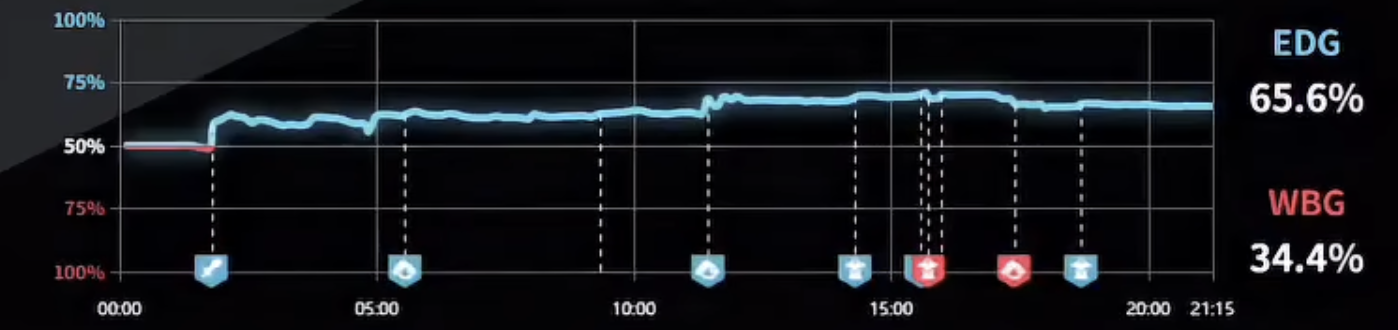
\includegraphics[width=\textwidth]{assets/edg_vs_wbg_g4_wp.png}
  \caption{Win Probability Prediction in 2023 LPL Worlds Regional Qualifier EDG vs WBG Game 4 \cite{bilibili-2023}}
  \label{fig:edg_vs_wbg_g4_wp}
\end{figure}


\begin{figure}[H]
  \centering
  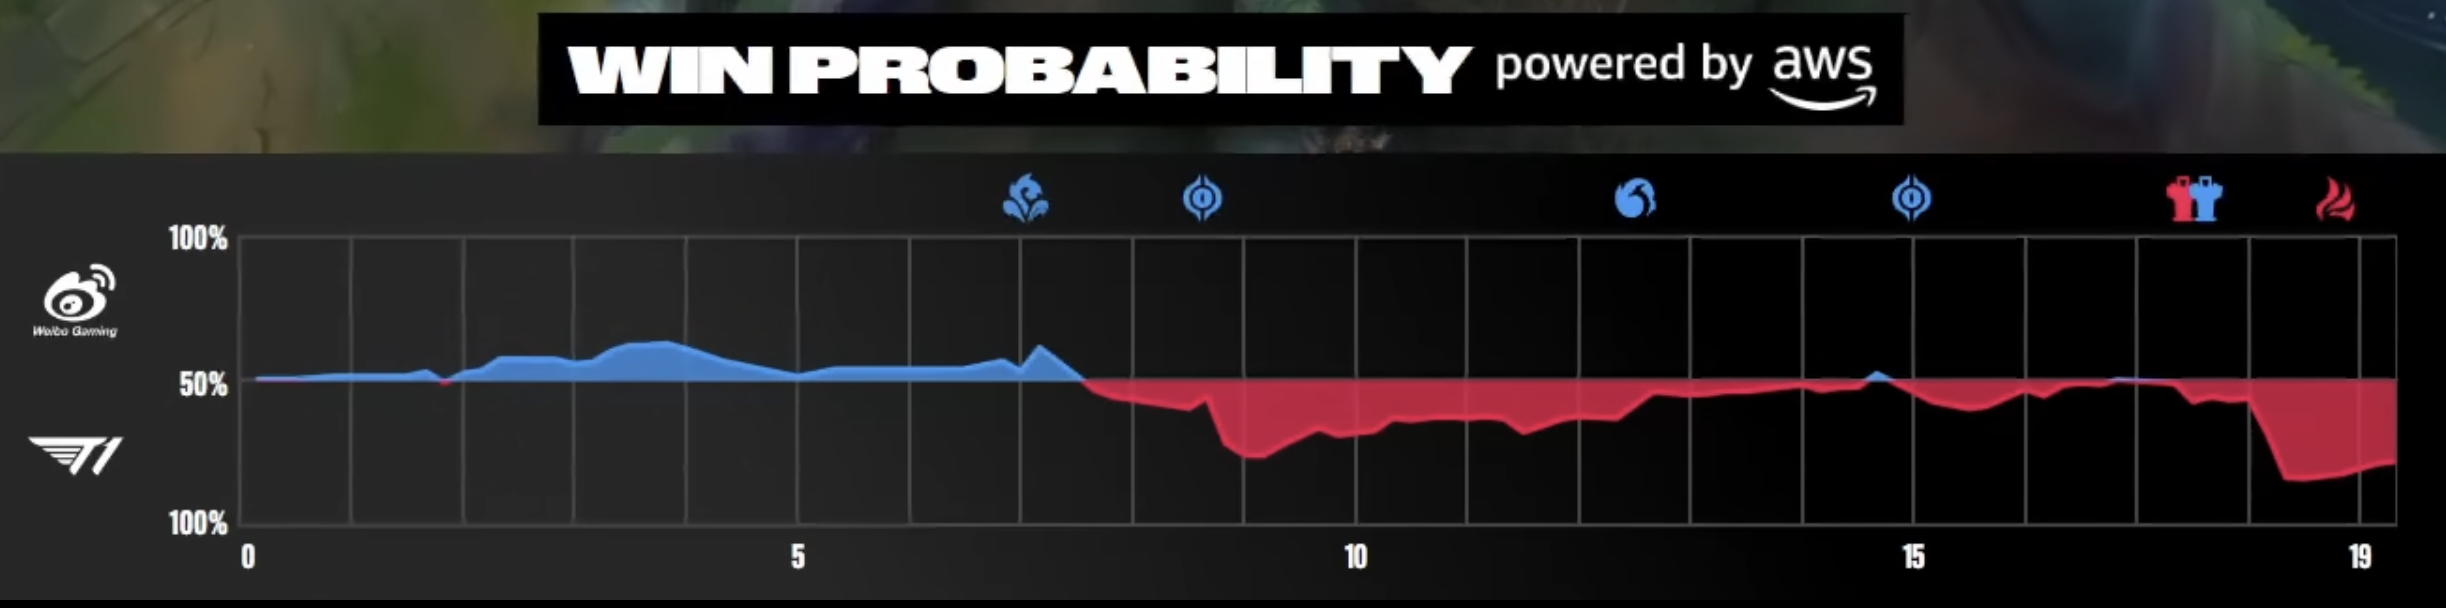
\includegraphics[width=\textwidth]{assets/t1_vs_wbg_g2_wp.png}
  \caption{Win Probability Prediction in Worlds 2023 Final WBG vs T1 Game 3 \cite{youtube-2023}}
  \label{fig:t1_vs_wbg_g2_wp}
\end{figure}

\begin{table}[H]
  \centering
  \caption{Factors that the LoL Esports WP XGBoost model takes into consideration \cite{lol-esports-2023}}
  \label{tab:lol_esports_factors}
  \begin{tabular}{cc}
    \hline
    \textbf{factor}                     & \textbf{note}                                     \\
    \hline
    Game time                           & the in-game time                                  \\
    Gold \%                             & player gold / total gold in game                  \\
    Total team XP                       &                                                   \\
    \# of players alive
                                        &                                                   \\
    Tower kills
                                        &                                                   \\
    Dragon kills
                                        & whether a team has dragon soul or not             \\
    Herald trinket in Inventory
                                        &                                                   \\
    Inhibitor timers for each inhibitor & how long until an inhibitor respawns              \\
    Baron timers                        & time until Baron buff expires for the team        \\
    Elder timer                         & time until Elder Dragon buff expires for the team \\
    \# of players with Baron active     &                                                   \\
    \# of players with Elder active     &                                                   \\
    \hline
  \end{tabular}
\end{table}

% \section{Riot Developer Policy}

% https://support-leagueoflegends.riotgames.com/hc/en-us/articles/225266848-Third-Party-Applications

\section{Riot API}
\label{sec:riot_api}

Riot Games offers a wide range of public APIs that provide access to game-related information for various purposes, beyond just League of Legends. The Riot Developer Portal, which can be found at \href{https://developer.riotgames.com/apis}{https://developer.riotgames.com/apis}, presents a user-friendly web interface accompanied by comprehensive documentation, as shown in Figure \ref{fig:riot_api}.

To access the APIs, you need to register a developer account on the portal and request an API key. The API key is refreshed every 24 hours. It's important to note that Riot Games enforces certain rate limits to maintain the stability of their services. The rate limit is set to 20 requests per 1 second and 100 requests per 2 minutes.

Riot provides valuable API endpoints to assist developers in their projects. For instance, the \texttt{account/v1} APIs allow us to find the unique player ID (called \texttt{puuid}) by using the player's game name and tag line. This can help us identify and track specific players. Additionally, the \texttt{match/v5} endpoints allow us to find matches of a player using either the match ID or the \texttt{puuid}. These APIs play a crucial role in this project as they are essential for collecting data to train machine learning models and develop applications.

\begin{figure}[H]
  \centering
  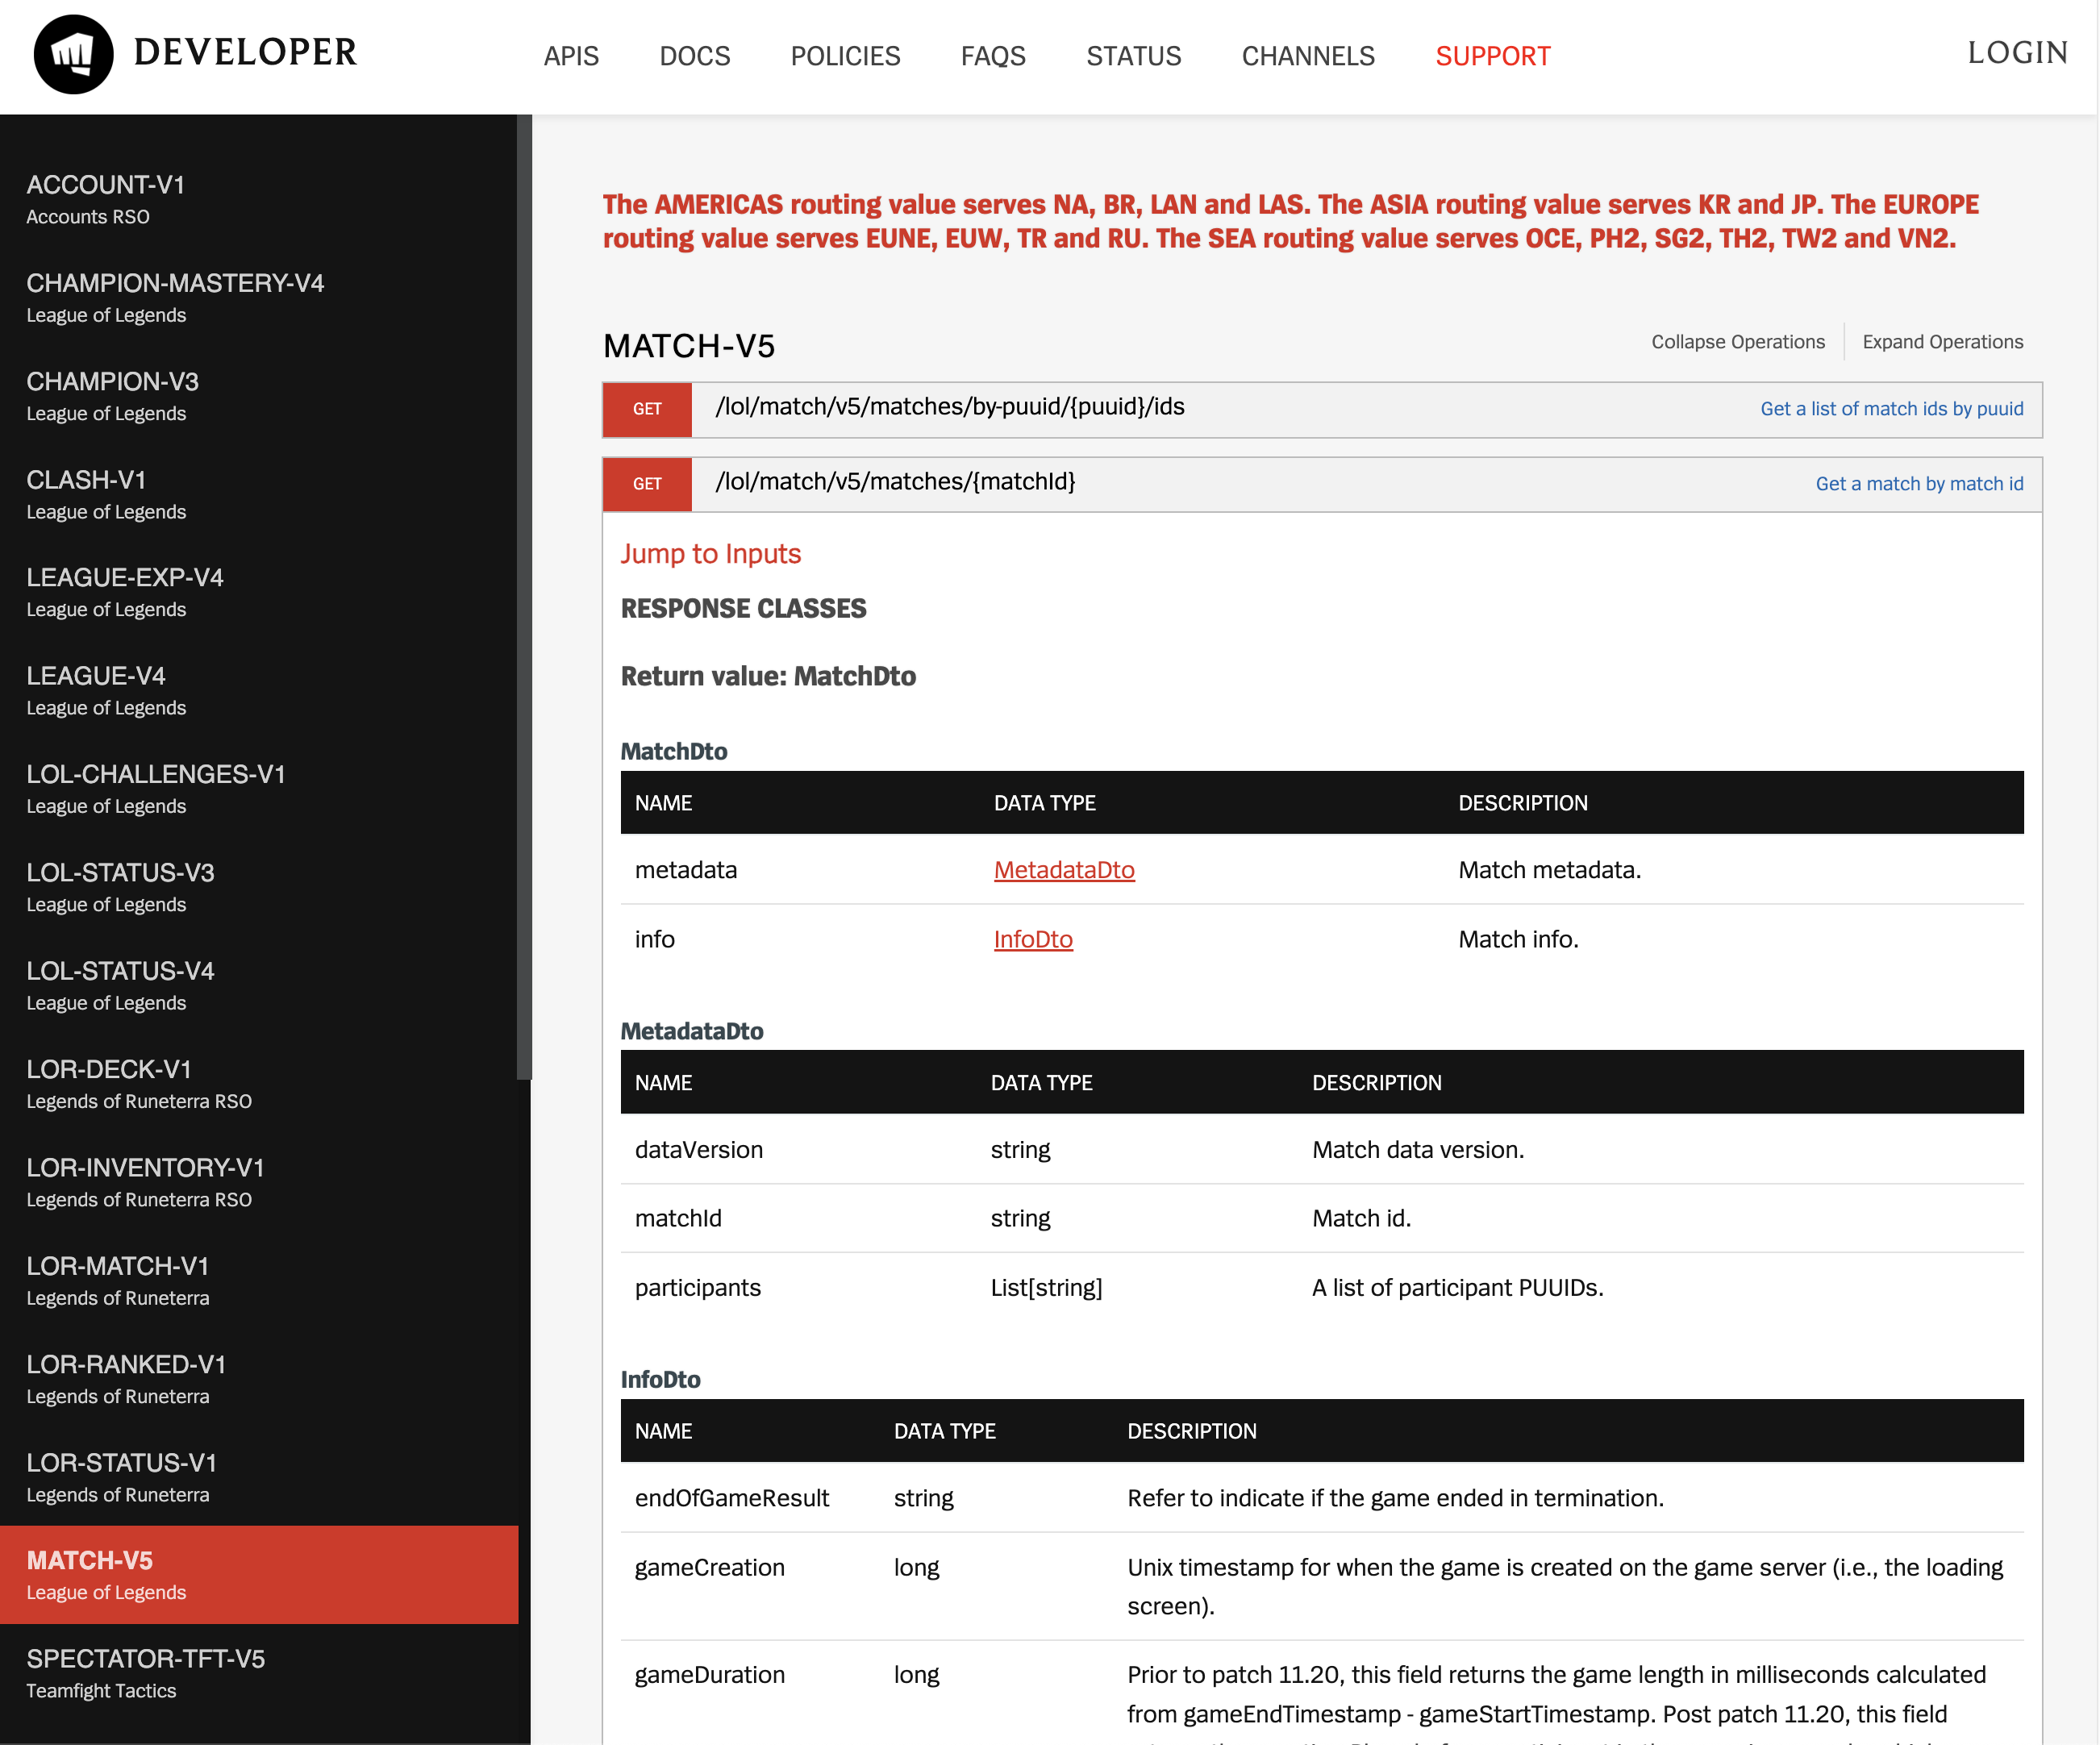
\includegraphics[width=0.8\textwidth]{assets/riot_api.png}
  \caption{\href{https://developer.riotgames.com/apis}{Riot API}}
  \label{fig:riot_api}
\end{figure}

As mentioned previously, League of Legends is developed and published by Riot Games. Riot directly operates the majority of regional servers, including NA, EUW, KR, JP, and TW. However, in China, League of Legends (as well as other games developed by Riot, such as \textit{Valorant}) is operated by \textit{Tencent}. Unlike Riot, Tencent does not provide publicly accessible APIs. Therefore, for our data collection in Chapter \ref{sec:data_preparation}, we focused on the KR server.

\section{League Client Update (LCU)}
\label{sec:lcu}

The League Client Update (LCU) refers to the revamped client for \textit{League of Legends}, introduced in 2016. Riot Games chose to call it a ``League Client Update'' because it represented a newer, more easily maintainable, and scalable software architecture.

In a blog post by Riot's software architects \cite{mc-veigh-2016}, they discussed the reasons behind moving away from the original client built with Adobe AIR in 2008, as well as an overview of the new architecture.

The original League of Legends client was built using Adobe AIR, which provided rich multimedia features but had its limitations. However, three key issues with the original client prompted the need for an update:

\begin{itemize}
  \item HTML5 Adoption: HTML5 emerged as a viable technology for desktop clients, offering standardized workflows and a larger pool of skilled developers.
  \item Connectedness: Players desired enhanced connectivity both within and outside the game, which the original client struggled to provide effectively, leading to excessive memory usage.
  \item Streamlined Software Development Management: As Riot Games expanded, multiple teams sought to add features to the client. However, the original codebase was designed for a small, tightly-knit team and did not offer the necessary level of autonomy and independence as the number of feature teams increased. To address this, a transition from monolithic software to microservices was required.
\end{itemize}

In the new architecture, Riot Games adopted the Chromium Embedded Framework (CEF) as the frontend, complemented by backend microservices written in C\texttt{++}. This approach involved presenting the asynchronous game protocol as a set of REST resources in backend microservices.

The use of JavaScript with CEF was chosen to ensure consistency by leveraging HTML5 and JavaScript. The C\texttt{++} backend microservices ran on the player's desktop and exposed the RTMP protocol as REST resources, reducing asynchronicity in the JavaScript code. Websockets were employed to handle events sent back to the user interface. This microservices layer was referred to as the ``foundation''. This design decision resulted in a more efficient client, as a significant portion of the backend business logic was implemented in C\texttt{++}, leading to a smaller memory footprint compared to a monolithic application.

The aforementioned components primarily focus on the communication between the game frontend and backend. The game backend, implemented in C\texttt{++}, communicates with the Riot datacenters since League of Legends is an online game. The C\texttt{++} backend handles events such as in-game chat, matchmaking, and queuing, interacting with the LoL platform and processing the results. The frontend then displays the updates to the user.

\begin{figure}[H]
  \centering
  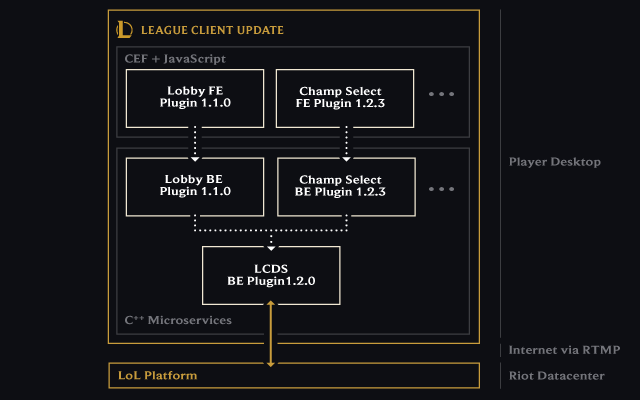
\includegraphics[width=0.8\textwidth]{assets/lcu_architecture.png}
  \caption{Overview of the LCU Architecture \cite{mc-veigh-2016}}
  \label{fig:lcu_architecture}
\end{figure}

The overall architecture of the League Client Update can be visualized as depicted in Figure~\ref{fig:lcu_architecture}. The game client is divided into two major components: the frontend, which utilizes CEF and JavaScript, consisting of frontend (FE) plugins, and the backend, composed of C\texttt{++} microservices and backend (BE) plugins. The frontend communicates with the backend through RTMP as REST resources. The C\texttt{++} microservices, in turn, communicate with the Riot datacenters by invoking remote calls via RTMP.

Official documentation for all LCU API endpoints (the REST resources provided by the C\texttt{++} microservices) is not provided by Riot. However, community efforts have made most of the LCU endpoints accessible. Tools like Rift Explorer \cite{pupix} and its successor LCU Explorer \cite{hextech-docs} offer a list of LCU endpoints in an application.

The LCU endpoints provide developers with opportunities to create their own applications, as long as they adhere to Riot's developer policy. For instance, the well-known statistics website OP.GG offers a desktop application that provides functionalities such as recommended items and runes for players. This application utilizes LCU endpoints under the hood, interacting with the game client through REST APIs. This project also includes a minimal pre-game win rate prediction application based on teammate information and team composition during the ban/pick phase, utilizing the LCU APIs.

In Chapter \ref{sec:rust_backend}, we will delve into methods of communicating with the LCU and explore how game prediction models work with data fetched from LCU endpoints.

% \section{Statistics Websites}

\section{Related Work}
\label{sec:related_work}

In the context of League of Legends, there are two types of win rate prediction: pre-game prediction and in-game prediction. These two types of machine learning models are the focus of our project.

\subsection{Pre-game Prediction}

The pre-game prediction typically utilize information that is known before the actual start of the game, as after the ban/pick phase. The ban/pick phase refers to the stage where players select their champions and bans champions that they consider they would be a trouble for them, and it is not considered part of the game phase itself. The rationale behind this approach is that players tend to estimate their likelihood of winning the game after the ban/pick phase based on factors such as their skills, team composition, and the power level of the selected champions in the current game version.

Do et al. \cite{do-wang-yu-mc-millian-mc-mahan-2021} developed pre-game prediction models that incorporate features like champion mastery points and player-champion win rates. They explored various machine learning models, including support vector machine classifiers, k-nearest neighbors, and deep neural networks. Similar implementations can also be found on GitHub \cite{reneleogp}, where pre-game data is utilized with different models. However, these models often do not take into account the strength of the chosen champions in the specific game version, which is a crucial factor as more powerful champions tend to have a higher likelihood of winning.

These machine learning models are primarily designed for research purposes, and there is currently no frontend application available for them. Applications like Record \cite{record} and Frank \cite{frank}, which have inspired this project, provide teammate information and statistics such as ranks and recent game results but do not offer win rate estimations. In this project, we aim to combine the two aspects: developing a machine learning model that predicts the pre-game win rate, and creating a frontend application that displays the predicted win rate along with other information, such as teammates' past game records. By integrating these components, we can provide users with an estimation of their win rate and additional relevant information to enhance their decision-making process before entering a game.

\subsection{In-game Prediction}

For in-game prediction, it is important that the machine learning model can provide ongoing estimations of the win rate as the game progresses. This is particularly relevant in the context of broadcasting LoL professional matches, where the current and previous game state is known, and the goal is to predict the win rate based on the game state up to that point.

In Chapter \ref{sec:lol_esports}, it was mentioned that developers in LoL Esports have built a win rate prediction model using XGBoost, a decision tree-based model. They utilize similar historical games to provide predictions for the current game, incorporating game time as a feature.

Chinicz developed both a machine learning model based on support vector machines and a frontend visualization for win rate prediction \cite{chinicz-2023}. However, their model oversimplifies the game state by considering only the end state of each game, disregarding the continuous sequence of game states throughout the match. This approach is less effective because in reality, predictions need to be made while the game is still in progress.

Junior \& Campelo \cite{junior-campelo-2023} created an in-game prediction model using LightGBM. They divided the game into four parts based on elpased time (20\% PET, 40\% PET, 60\% PET, and 80\% PET) to account for different feature importance in different game stages \cite{junior-campelo-2023}. They trained a LightGBM model for each stage and explored feature importance within those portions of the game. While analyzing feature importance in different stages is meaningful, building different models for different stages of a game can be cumbersome and lead to inconsistencies.

Jang et al. \cite{jang-woo-kim-2022} proposed a novel embedding model that quantifies a player's actions based on their contribution to the team's victory, using Gated Recurrent Unit (GRU). Their model provides an novel way to assess value of a player's action. However, their model processes the entire sequence data of the game, making it unsuitable for real-time in-game prediction, as it requires data from the entire match.

Due to the sequential nature of the LoL game state, we decided to use a Long Short-Term Memory (LSTM) model for in-game prediction. The LSTM model is capable of capturing temporal dependencies in the features and can be used to predict the win rate at any given time in the game, leveraging the historical context up to that point. This approach allows for real-time predictions and takes advantage of the LSTM's ability to model sequential data effectively.

%%%%%%%%%%%%%%%%%%%%%%%%%%%%%%%%%%%%%%%%%%%%%%%%%%%%%%%%%%%%%%%%%%%%%%%%%%%%%%%%

% \chapter{Material and Methods}
% \label{material-and-methods}

\instructions{This section is obviously discipline specific so use the
  nomenclature that is common for your discipline. However, this section
  should provide sufficient detail about the materials and the methods
  used so that other experienced workers can repeat the experiment and
  obtain comparable results. Cite the appropriate literature when using a
  standard method or protocol and give only the details needed. Identify
  the materials used in the research. For example, computer systems used,
  mathematical theorems exploited, etc.; give information on the purity of
  all chemicals and reagents employed in the research; include the
  chemical/biological names of all compounds and chemical formulas of
  substances that are new or uncommon. Use standard systematic
  nomenclature to unambiguously define well-established compounds,
  processes, equipment, etc.}

%%%%%%%%%%%%%%%%%%%%%%%%%%%%%%%%%%%%%%%%%%%%%%%%%%%%%%%%%%%%%%%%%%%%%%%%%%%%%%%%

% \chapter{Results}
% \label{results}

\instructions{Summarize the data collected in this section, and their
  statistical treatment. Include only relevant data, but give sufficient
  detail to justify the conclusions. It is appropriate in this section to
  use equations, figures, and tables to display your data. Extensive, but
  relevant data, should be reserved for an appendix where it is identified
  as supporting information.}

\instructions{The table or figure must follow as closely as possible after the
  paragraph in which it is referenced. Titles/captions should be kept
  brief.}

% \section{Examples}

% Here is some inline math, $x^2 > 1$, and some display math
% \begin{equation}
%   \int_0^1 x^2 \, dx
% \end{equation}
% And this is how to cite an article \cite{Zhang2021} or a book \cite{Axler2020}.

% \begin{table}[htbp]
% \centering
% \begin{tabular}{@{}llll@{}}
% \toprule
% \emph{Replace} & \emph{With} & \emph{Your} & \emph{Table} \\
% \midrule
% & & & \\
% & & & \\
% \bottomrule
% \end{tabular}
% \caption{Parameters for the optimization of the principal component analysis for
% olive oil adulteration.}
% \label{tbl:2}  
% \end{table}


% \begin{figure}[htbp]
% \centering
% \includegraphics[height=4cm]{btc.jpg}
% \caption{The notorious BTC (Brandon The Cat).}
% \label{fig:1}
% \end{figure}

%%%%%%%%%%%%%%%%%%%%%%%%%%%%%%%%%%%%%%%%%%%%%%%%%%%%%%%%%%%%%%%%%%%%%%%%%%%%%%%%

% \chapter{Discussion}
% \label{discussion}

\instructions{The discussion section is where you interpret and compare the
  results. The objective is to point out the features and limitations of
  the work. Relate your results to current knowledge in the field and to
  the original purpose for undertaking the project.}

%%%%%%%%%%%%%%%%%%%%%%%%%%%%%%%%%%%%%%%%%%%%%%%%%%%%%%%%%%%%%%%%%%%%%%%%%%%%%%%%

\chapter{Architecture Overview}
\label{architecture_overview}

This project encompasses two applications: pre-game prediction and in-game prediction. This chapter provides an overview of the architecture and workflow of the entire project, including training data preparation, the machine learning backend, and the two applications that leverage machine learning.

\section{Training Data Preparation}

\subsection{Riot API}

To gather data for training, we utilized the Riot API \cite{riot-api} to collect timeline data from approximately 2000 games. This continuous timeline data comprises various in-game events and serves as the foundation for training the LSTM model. Additionally, we collected game data related to champion mastery of each player, which is utilized for pre-game prediction.

\subsection{Web Scraping}

In addition to the Riot API data, we collected game-related information from statistics websites such as \href{https://www.op.gg/}{OP.GG}. These websites provide valuable insights into factors such as overall champion win rates, win rates over time, champion counter relationships, and the impact of champion item builds on win rates. While conducting these statistics ourselves would be ideal, the limited sample size of only 2000 games prevents us from obtaining comprehensive and statistically significant results.

\section{Machine Learning Backend}

Machine learning is the core of this project, below is an overview of the two tasks, we will continue to discuss the details in Chapter \ref{sec:pre-game_prediction_model} and \ref{sec:in-game_prediction_model}.

\subsection{Pre-game Prediction}

For pre-game prediction, we employ a machine learning approach that utilizes several factors for logistic classification. These factors include the past performance of teammates in their previous 5 games, their champion mastery levels, and champion statistics data. By considering these variables, we aim to make informed predictions about the outcome of the upcoming game.

\subsection{In-game Prediction}

In the case of in-game prediction, we utilize a concept similar to word2vec  \cite{word2vec} to measure the compatibility between a champion and an item. To achieve this, we incorporate various game-related features into the training of our LSTM model. These features encompass gold, gold differential, experience (exp), experience differential, turrets, heralds, Baron Nashor, drake kills, champion overall win rate, champion win rate at a specific minute, and the compatibility between a champion and an item.

\section{Applications Leveraging Machine Learning}

We have developed two applications that correspond to pre-game and in-game prediction.

\subsection{Pre-game Prediction Application}

The pre-game prediction application is built using the Tauri \cite{tauri} framework, which combines Rust \cite{rust} for the backend and React \cite{react} with Typescript \cite{type-script} for the frontend. The Rust backend communicates with the League Client (LCU) to retrieve champion selection data during the ban/pick phase. This data is then processed and utilized for prediction purposes. On the frontend, the React application displays the past game records of teammates and showcases the pre-game predictions generated by the backend.

\subsection{In-game Prediction Application}

For the in-game prediction application, we utilize React along with D3.js \cite{d3} to visualize the trend of win rates. In this setup, a local Flask \cite{flask} server is employed to read real-time timeline data from the League Client in spectator mode. The Flask server processes this data and publishes predictions based on the ongoing game. The React frontend application reads these predictions and displays them using D3.js. The win rate trend can be displayed as an \href{https://obsproject.com/}{OBS} overlay.

%%%%%%%%%%%%%%%%%%%%%%%%%%%%%%%%%%%%%%%%%%%%%%%%%%%%%%%%%%%%%%%%%%%%%%%%%%%%%%%%

\chapter{Implementation Details}
\label{implementation_details}

\section{Data Preparation}
\label{sec:data_preparation}
\subsection{Riot Api}

As outlined in Chapter \ref{sec:riot_api}, we utilized the Riot API to gather a significant portion of the data required for training our machine learning models. Specifically, we collected approximately 2000 games from the Korea server by making use of the following endpoints: \\ \texttt{/lol/match/v5/matches/{matchId}} and \texttt{/lol/match/v5/matches/{matchId}/timeline}.

The first endpoint provided us with general information about each game, including details such as the game mode, participants, and the final result. In contrast, the timeline data consisted of game events that occurred at each minute, rendering it a sequential dataset. To prepare this data for training the in-game prediction model detailed in Chapter \ref{sec:in-game_prediction_model}, we performed several data preprocessing steps. This involved aggregating specific game events, such as monster kills and turret takedowns, to ensure that the resulting timeline data was suitable for training purposes.

Additionally, we retrieved a list of matches by \texttt{puuid} utilizing the endpoint \\ \texttt{/lol/match/v5/matches/by-puuid/{puuid}/ids}. Furthermore, we obtained champion mastery data using the \texttt{champion-mastery/v4} endpoints. These datasets were used in training the pre-game prediction model described in Chapter \ref{sec:pre-game_prediction_model}.

By leveraging the Riot API and collecting data from various endpoints, we were able to acquire the necessary information to train our pre-game and in-game prediction models effectively. This data will serve as a foundation for the subsequent chapters, where we delve into the specifics of each model and their respective training processes.

% \subsection{Statistics Websites}

% \subsection{Riot Api vs LCU}

% \subsubsection{Headless Chrome}

% \subsubsection{BeautifulSoup4}

% \subsubsection{Selenium}

\subsection{Game Assets}

The game timeline data obtained from the Riot API may not include all the necessary information, requiring us to find the missing details. For instance, the timeline data often provides identifiers (IDs) for various entities such as champions, items, and runes. To make this data more meaningful, we need to map these IDs to their corresponding properties. To accomplish this, we rely on Data Dragon, commonly referred to as DDragon, which is a collection of static data files containing information and images for champions, runes, and items \cite{ddragon}. DDragon enables us to translate champion IDs into their respective names and provides additional details for other entities.

Furthermore, the timeline data obtained from the spectator mode in the in-game prediction application from Chapter \ref{sec:in-game_prediction_application} does not include the total gold accumulated by each player. To address this, we approximate the total gold by summing up the prices of the items owned by each player. For this purpose, we require the item details from DDragon.

In addition to the data used for training our machine learning models, we have also prepared various game assets such as champion and item icons for the frontend applications.

\section{Pre-game Prediction Model}
\label{sec:pre-game_prediction_model}

\subsection{Feature Engineering and Preprocessing}

In our pre-game prediction model, we extract relevant information that is available before the start of a game. This refers to the period after the ban/pick phase but before the actual gameplay begins, as discussed in Chapter \ref{sec:related_work}.

We use features listed in Table \ref{tab:pre_game_features} to train the pre-game prediction model. Champion Mastery is a progression system which tracks a player's aptitude and experience with each champion \cite{lol-wiki-champ-mastery}. KDA is also an metrics assessing a player's performance, as mentioned in Chapter \ref{sec:game_topics}.

\begin{table}[htbp]
  \centering
  \caption{Features used in the pre-game win rate prediction model}
  \label{tab:pre_game_features}
  \begin{tabular}{cc}
    \hline
    \textbf{Features}                         \\
    \hline
    Sum of champion mastery                   \\
    Sum of KDA in past 5 games                \\
    Current pick champion win rate from OP.GG \\
  \end{tabular}
\end{table}

\subsection{Logistic Regression}

We use a logistic regression model for our pre-game prediction task. To implement this model, we leverage the logistic regression implementation provided by scikit-learn \cite{sklearn-logistic-regression}, which incorporates $L_2$ regularization.

\subsection{Experiment Results}

To evaluate the performance of our pre-game prediction model, we partitioned the dataset, reserving 30\% as a test set. The logistic regression model achieved an accuracy of 73.5\% on the training set and 70.3\% on the test set, demonstrating its ability to predict win rates based on pre-game information.

\section{In-game Prediction Model}
\label{sec:in-game_prediction_model}

\subsection{Feature Engineering}
\subsubsection{Champion-Item Compatibility and Preprocessing}
\label{sec:embedding}
We utilized data scraped from the statistics website \href{https://www.op.gg/}{OP.GG} to obtain champion builds and item statistics. OP.GG provides valuable information such as the pick rate and win rate of specific items for each champion. Figure \ref{fig:opgg_caitlyn_builds} illustrates an example where most Caitlyn players choose the item \textit{Infinity Edge}, which is crucial for champions reliant on critical strikes. Additionally, the item with the highest win rate for Caitlyn is \textit{Guardian Angel}, as it offers defensive effects, and players tend to select this item when they have an advantage.

While it would be ideal to collect and analyze comprehensive statistics ourselves, the limited sample size of only 2000 games prevents us from obtaining statistically significant results. Moreover, certain champions are more popular and appear more frequently in our dataset, while others are rare sightings. Additionally, players have diverse playstyles and may opt for different item builds. These factors introduce biases into our dataset. To mitigate this, we rely on data from large statistics websites like \href{https://www.op.gg/}{OP.GG} to ensure more accurate and representative statistics for our predictions and insights.

Given a champion vector $\mathbf{c}$ and an item vector $\mathbf{i}$, where $\mathbf{c}, \mathbf{i} \in \mathbb{R}^d$, their compatibility is modeled using the cosine similarity:

\[\frac{\mathbf{c}^T\mathbf{i}}{\|\mathbf{c}\| \|\mathbf{i}\|} \in [-1, 1]\]

\begin{figure}[htbp]
  \centering
  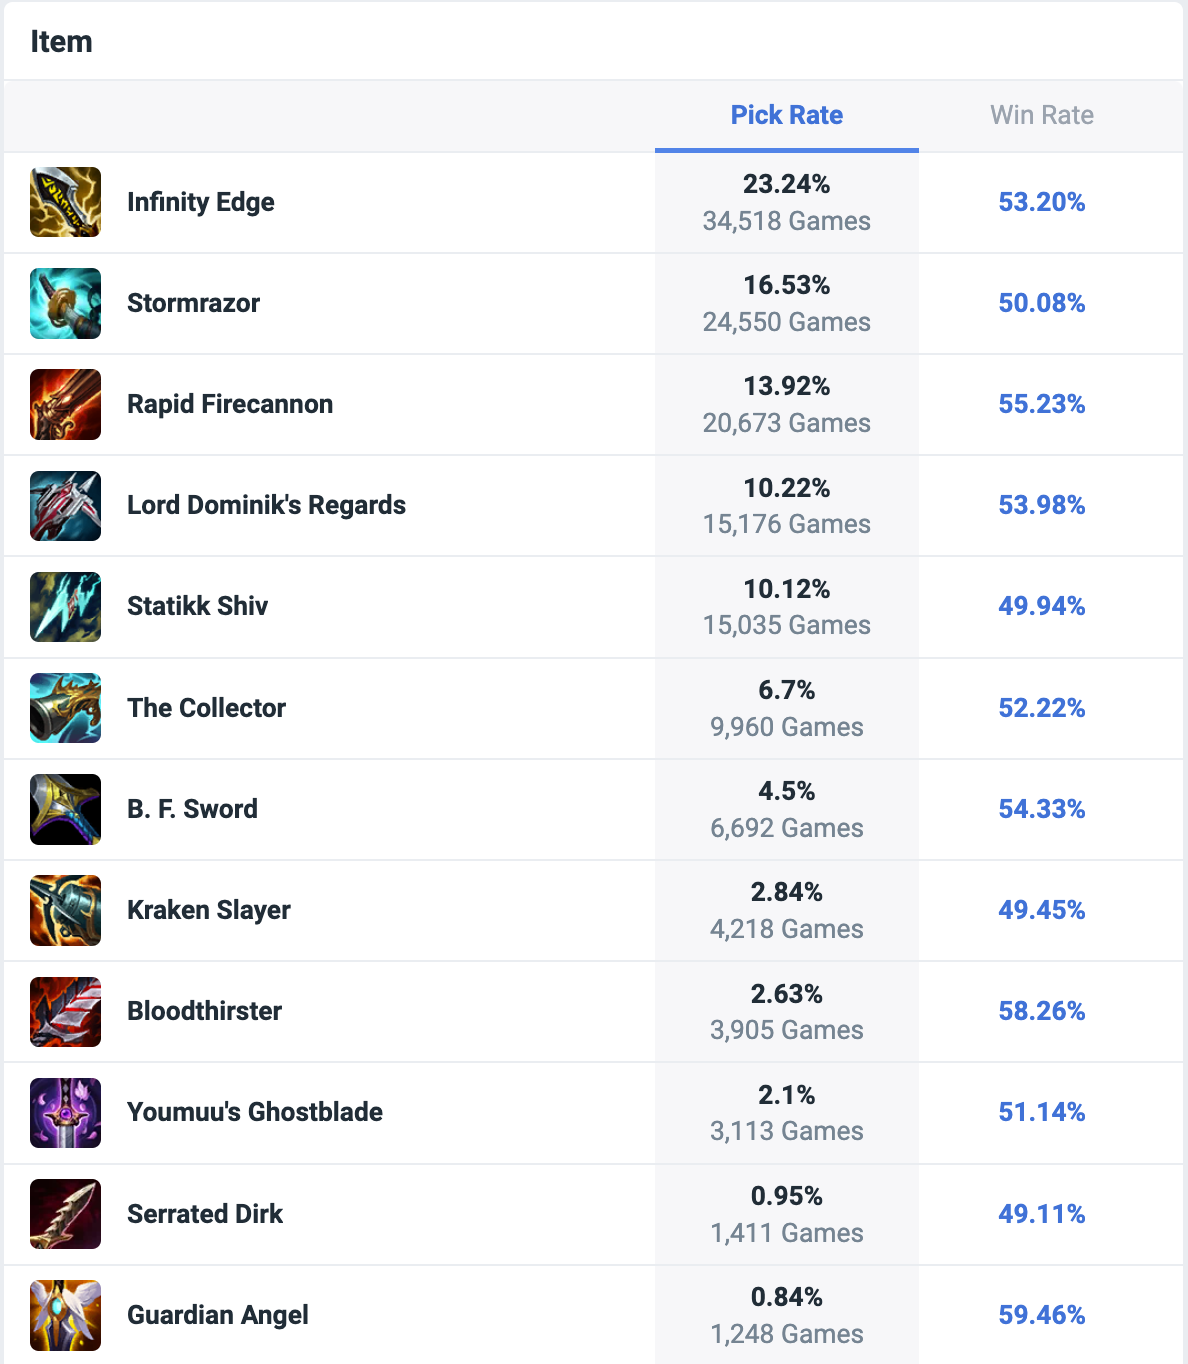
\includegraphics[height=0.45\textheight]{assets/opgg_caitlyn_builds.png}
  \caption{Caitlyn item builds on \href{https://www.op.gg/}{OP.GG} \cite{opgg-caitlyn-builds}}
  \label{fig:opgg_caitlyn_builds}
\end{figure}

To assign a score to a champion-item pair, we utilize the pick rate $p_0$ and win rate $p_1$ with the following formula:

\[\text{Score} = ((\frac{p_0}{75})^2 + v_1)^2 \]

This formula is based on two assumptions:

\begin{itemize}
  \item Items with higher pick rates should have higher scores.
  \item Items with a low sum of pick rate and win rate should be penalized, hence the quadratic function to discourage small scores.
\end{itemize}

We model coexistence between the champion set $S$ and the item set of each champion $S_j$, where $j$ represents a champion and $w_{jk}$ denotes the score between champion $j$ and item $k$:

\[\text{Loss} = \sum_{j \in S}\sum_{k \in S_j} w_{jk}\text{BCE}(\sigma(\mathbf{c}_j^T\mathbf{i}_k), 1)\]

The loss function aims to increase the value for champion-item pairs with high scores, encouraging better compatibility.

\begin{figure}[htbp]
  \centering
  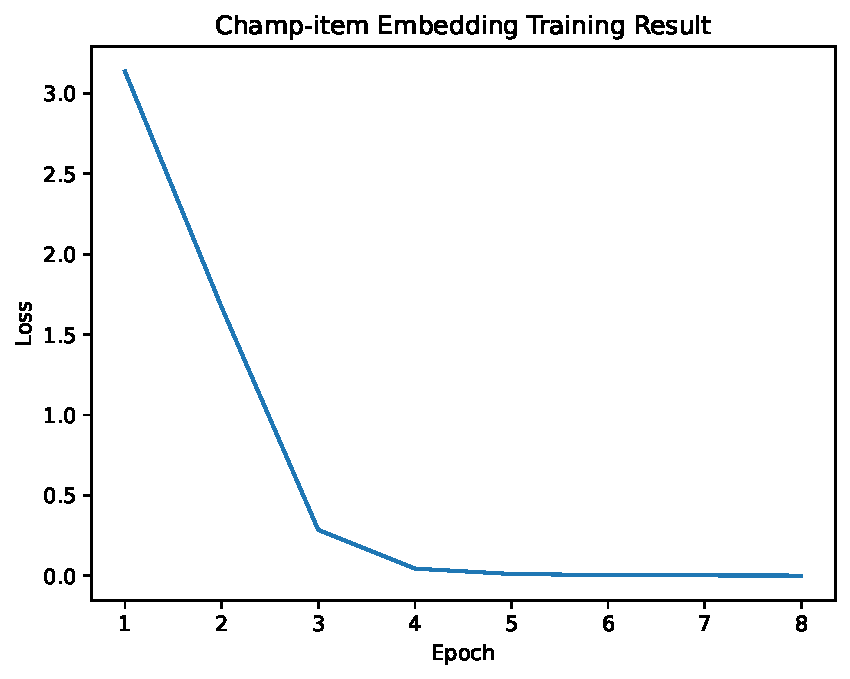
\includegraphics[height=0.4\textheight]{assets/champ-item_embedding_training_result.pdf}
  \caption{Champion-item embedding training result}
  \label{fig:champ-item_embedding_training_result}
\end{figure}

Although the primary focus of this project is champion-item compatibility, the champion-item embedding provides additional valuable information. Similar to word embedding models, we can extract champion patterns and item patterns from the embeddings.

For instance, when querying the top 10 champions similar to the champion \textit{Aatrox}, we obtain the following results:

\begin{verbatim}
cosine sim=1.000: Aatrox
cosine sim=0.995: Nocturne
cosine sim=0.993: Wukong
cosine sim=0.992: Kled
cosine sim=0.991: Vi
cosine sim=0.990: Viego
cosine sim=0.990: Briar
cosine sim=0.989: Yorick
cosine sim=0.987: Riven
cosine sim=0.987: Kayn
\end{verbatim}

The results are quite impressive, as all these champions are sustained fighters similar to Aatrox.

Similarly, when querying the top 10 items similar to \textit{Thornmail}, we obtain the following results:

\begin{verbatim}
cosine sim=1.000: Thornmail
cosine sim=0.998: Bramble Vest
cosine sim=0.988: Spirit Visage
cosine sim=0.988: Iceborn Gauntlet
cosine sim=0.987: Randuin's Omen
cosine sim=0.986: Jak'Sho, The Protean
cosine sim=0.984: Dead Man's Plate
cosine sim=0.983: Frozen Heart
cosine sim=0.982: Kaenic Rookern
cosine sim=0.979: Force of Nature
\end{verbatim}

However, during the process of querying items that are a good fit for Aatrox, an unexpected result of \textit{Muramana} surfaced. This is surprising because Aatrox does not have mana, and Muramana is specifically designed for champions with mana.

\begin{verbatim}
cosine sim=0.994: Death's Dance
cosine sim=0.992: Executioner's Calling
cosine sim=0.992: Black Cleaver
cosine sim=0.991: Profane Hydra
cosine sim=0.991: Tiamat
cosine sim=0.990: Chempunk Chainsword
cosine sim=0.989: Eclipse
cosine sim=0.988: Sterak's Gage
cosine sim=0.986: Hullbreaker
cosine sim=0.983: Stridebreaker
cosine sim=0.983: Spear of Shojin
cosine sim=0.982: Ravenous Hydra
cosine sim=0.982: Sundered Sky
cosine sim=0.975: Muramana
\end{verbatim}

This anomaly occurs because Muramana is similar to other items that are suitable for Aatrox, causing them to be close in the embedding space. However, the model fails to learn that Aatrox cannot utilize Muramana due to the absence of mana. In future work, we can consider incorporating negative sampling in the embedding model to enhance the robustness of champion-item fitness results.

To make the model more holistic, we can incorporate runes as additional features. Runes play a crucial role in a player's strategy and can significantly impact the outcome of a game. By including rune information in our model, we can capture this important aspect and potentially improve the accuracy of our embedding model.

The features used in the in-game win rate prediction model are shown in Table \ref{tab:lstm_features}.

\begin{table}[htbp]
  \centering
  \caption{Features used in the in-game win rate prediction model}
  \label{tab:lstm_features}
  \begin{tabular}{cc}
    \hline
    \textbf{Features}                      \\
    \hline
    Team gold                              \\
    Gold difference                        \\
    Team experience                        \\
    Experience difference                  \\
    Turrets taking down                    \\
    Heralds kills                          \\
    Baron Nashor kills                     \\
    Drake kills                            \\
    Champion overall win rate              \\
    Champion win rate at a specific minute \\
    Champion-item fitness                  \\
  \end{tabular}
\end{table}

\subsection{Long Short-Term Memory (LSTM)}

The \textbf{Long Short-Term Memory} (LSTM) is a type of neural network specifically designed to handle sequential data, making it suitable for analyzing the sequential game timeline information. LSTMs are commonly used in deep learning for tasks involving sequence prediction. Given the nature of our data, which consists of game states observed at different minutes, LSTM is well-suited for capturing temporal dependencies and patterns.

To construct our LSTM model, we utilize the 11 features outlined in Table \ref{tab:lstm_features}, which cover various aspects of the game state.

The LSTM model architecture, implemented using the PyTorch library \cite{pytorch-lstm}, is defined as follows:

\begin{verbatim}
LSTM(
  (lstm): LSTM(11, 50)
  (linear): Linear(in_features=50, out_features=1, bias=True)
)
\end{verbatim}

In this architecture, our model takes a sequence of game timelines as input. Each time step in the sequence represents the game state at a specific minute. For instance, in a 25-minute game, the input shape would be (25, 11), indicating 25 time steps and 11 features. The LSTM layer within the model has 50 hidden state features, allowing it to capture complex relationships and patterns in the data over time. After the LSTM layer, the output is passed through a linear layer with a sigmoid activation function. This final layer produces a single output, representing the predicted win probability for the team.

By leveraging the power of LSTM, our model can effectively analyze the sequential nature of the game timeline data and make predictions based on the historical information. The LSTM's ability to capture temporal dependencies enables it to learn from past game states and generate accurate win rate predictions for the team.

\subsection{Experiment Results}

Based on the provided information, the model was trained using approximately 2000 games of varying lengths in League of Legends. As the duration of a typical game in League of Legends can range from 15 to 40 minutes, a window size of 15 minutes was chosen for the sequence data. This window size allows for capturing relevant historical information and simplifies the training process.

\begin{figure}[htbp]
  \centering
  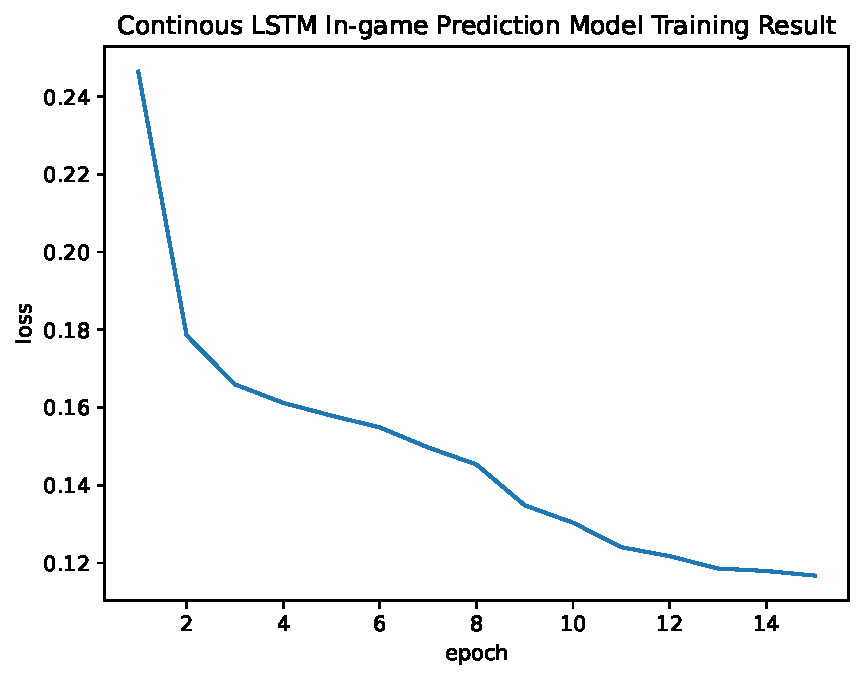
\includegraphics[height=0.4\textheight]{assets/lstm_train_accuracy.pdf}
  \caption{Continous LSTM in-game prediction model training result}
  \label{fig:lstm_train_accuracy}
\end{figure}

To evaluate the model's performance, tests were conducted using sequence data that covers the first $n$ minutes of a game, where $n$ represents the game time. This approach aligns with the in-game prediction application setting, where all past game states are considered. The tests involved game timelines ranging from 1 to 30 minutes. For instance, a first 15 minute timeline would correspond to a feature shape of \texttt{(15, 11)}.

As the length of the sequence increases, the model demonstrates improved performance due to its ability to account for complex temporal dependencies in the game. Moreover, the game result becomes more evident as time progresses, leading to more accurate predictions.

\begin{figure}[htbp]
  \centering
  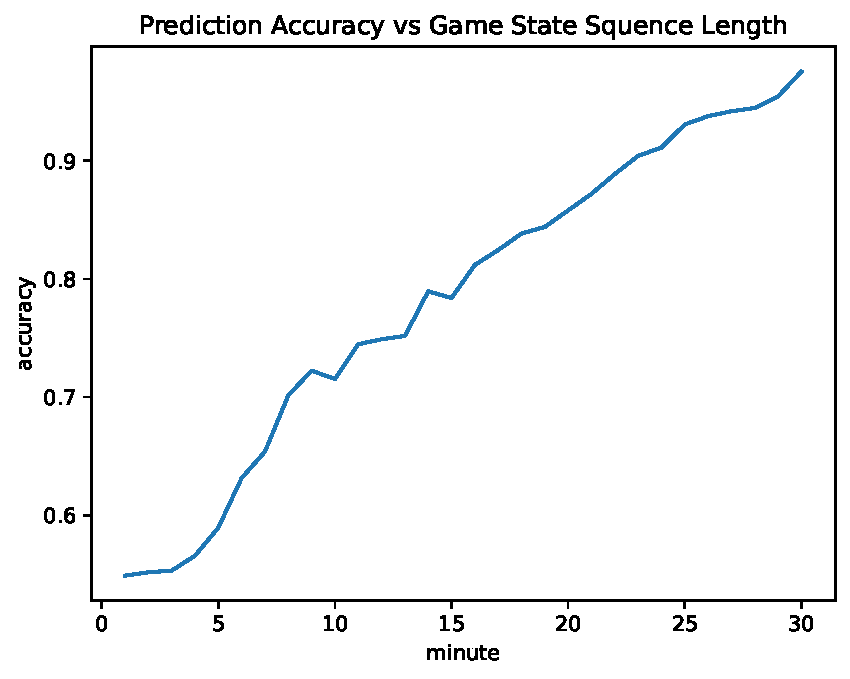
\includegraphics[height=0.4\textheight]{assets/lstm_test_accuracy.pdf}
  \caption{Prediction accuracy vs game state squence length}
  \label{fig:lstm_test_accuracy}
\end{figure}

Based on the results shown in the Figure \ref{fig:lstm_test_accuracy}, we observed that when using a sequence covering the first 30 minutes of a game, the model achieved an impressive prediction accuracy of 97\%, while it does perform as good in an early game due to the reasons mentioned above.

\section{Applications Leveraging Machine Learning}

\subsection{Pre-game Prediction Application}
\subsubsection{Rust Backend}
\label{sec:rust_backend}

As described in Chapter \ref{sec:lcu}, the League Client exposes an asynchronous game protocol through a set of REST resources in backend microservices. In this chapter, we will focus on the communication with the League Client using REST APIs. To establish communication with the League Client, we need to determine the port on which the League Client is listening and obtain the authentication token required for communication.

To retrieve the necessary information, we can inspect the command-line arguments of the League Client process, specifically the \texttt{LeagueClientUx.exe} executable \cite{ray-2022}. In PowerShell, we can find the command-line arguments, including the \texttt{remoting-auth-token} and \texttt{app-port} used for communicating with the LCU, by using the following commands:
\begin{verbatim}
$ $processName = "LeagueClientUx.exe"
$ $process = Get-WmiObject -Query "SELECT CommandLine FROM Win32_Process WHERE\
  Name = '$processName'" -ErrorAction SilentlyContinue
$ $process.CommandLine
> e:/path/to/LeagueClient/LeagueClientUx.exe ...... "--remoting-auth-token=dEcv\
> CiXBK3bO1ibvDlDsig" "--app-port=64325" ......
\end{verbatim}

In our project, we utilized the ``sysinfo'' Rust crate and the ``psutil'' Python package to retrieve this information. These libraries provide convenient functionalities to access process information and retrieve command-line arguments.

When communicating with the League Client's REST server, it's important to note that the League of Legends client and the game client utilize a self-signed certificate for HTTPS requests. To ensure secure communication, we need to use \href{https://static.developer.riotgames.com/docs/lol/riotgames.pem}{Riot's root certificate} to validate the game client's SSL certificate. Riot provides its root certificate, which can be obtained from the developer guide \cite{riot-lol-docs}.

To authenticate with the League Client, the \texttt{remoting-auth-token} needs to be prefixed with \texttt{riot:} and then encoded using Base64. Once encoded, we can add an \texttt{authorization: Basic <encoded-base64-token>} header to our requests, enabling successful communication wit hthe League Client's REST server.

In our Tauri application, we utilize the API endpoint from LCU \\\texttt{/lol-champ-select/v1/session} to retrieve teammate information and ban/pick details during the ban/pick phase. This API call is exposed as a command that the React frontend invokes. Additionally, our Rust backend implements several essential API calls, including retrieving player information by their unique ID (\texttt{puuid}) and fetching the player's game history based on the \texttt{puuid}.

In our application, the Rust backend handles the necessary data preparation for the pre-game win rate prediction model. It organizes the data into the required format for the model and then executes the prediction model, which is implemented in Python. The Rust backend makes the machine learning prediction available to the React frontend by exposing it as a command. This allows the React frontend to request the prediction and display it to the user.

\subsubsection{React Frontend}

The React frontend interacts with the Rust backend by invoking the implemented commands. It retrieves teammate information and ban/pick data from the Rust backend and displays this information using JSX/TSX \cite{react-jsx}, which allows for the rendering of dynamic components. Additionally, the React frontend calls the Rust backend to execute the pre-game win rate prediction model in Python and presents the resulting prediction to the user interface.

\begin{figure}[htbp]
  \centering
  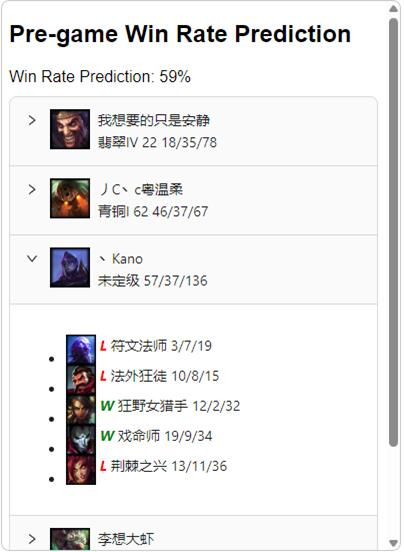
\includegraphics[height=0.4\textheight]{assets/pre_game_pred.jpg}
  \caption{Pre-game Prediction Application}
  \label{fig:pre_game_pred}
\end{figure}

\subsection{In-game Prediction Application}
\label{sec:in-game_prediction_application}
\subsubsection{Flask Machine Learning Backend}

In our system, we utilize the Live Client Data API to retrieve real-time game data. This API provides data that is available to us depending on the mode we are in. When in playing mode, we have access to data on our side and limited information about the opponents. In spectator mode, we have access to more comprehensive data. The in-game prediction, which is used in esports events, is specifically designed for spectator mode.

To retrieve real-time data, our Flask application makes requests to the endpoint \\ \texttt{https://127.0.0.1:2999/liveclientdata/activeplayer}. However, this API does not provide individual gold or team total gold information, which is crucial for running the in-game prediction model. Although providing such information in spectator mode is safe, Riot does not include it in the API response. LeagueBroadcast \cite{floh22} employs \textbf{direct memory access} (DMA) to access additional data in spectator mode, but we do not have access to that technology. It's worth noting that DMA is generally considered cheating, although it should be acceptable in spectator mode. As a result, we had to find an alternative solution. While we lack access to individual gold, we can still retrieve player item information. We approximate player gold by summing up the prices of their items. Since this approach is not perfect, we can explore how DMA works in LeagueBroadcast \cite{floh22} to obtain more accurate real-time game data in the future.

Once we have the real-time game data, our Flask application performs various data processing tasks, including the previously mentioned gold approximation. It then runs the LSTM in-game win rate prediction model. The LSTM model expects time sequence data as input, so the Flask application keeps track of the previous game states as \textit{context}. At regular intervals, the Flask application runs the inference using the model and publishes the prediction to a port on localhost. The React frontend overlay reads the prediction from that port and displays it to the user interface.

\subsubsection{Frontend Overlay}

The Frontend Overlay is a web application developed using React and D3.js. Its main functionality is to retrieve predictions from a Flask machine learning backend and present them as a line chart. The application periodically fetches the predictions and updates the chart accordingly.

\begin{figure}[htbp]
  \centering
  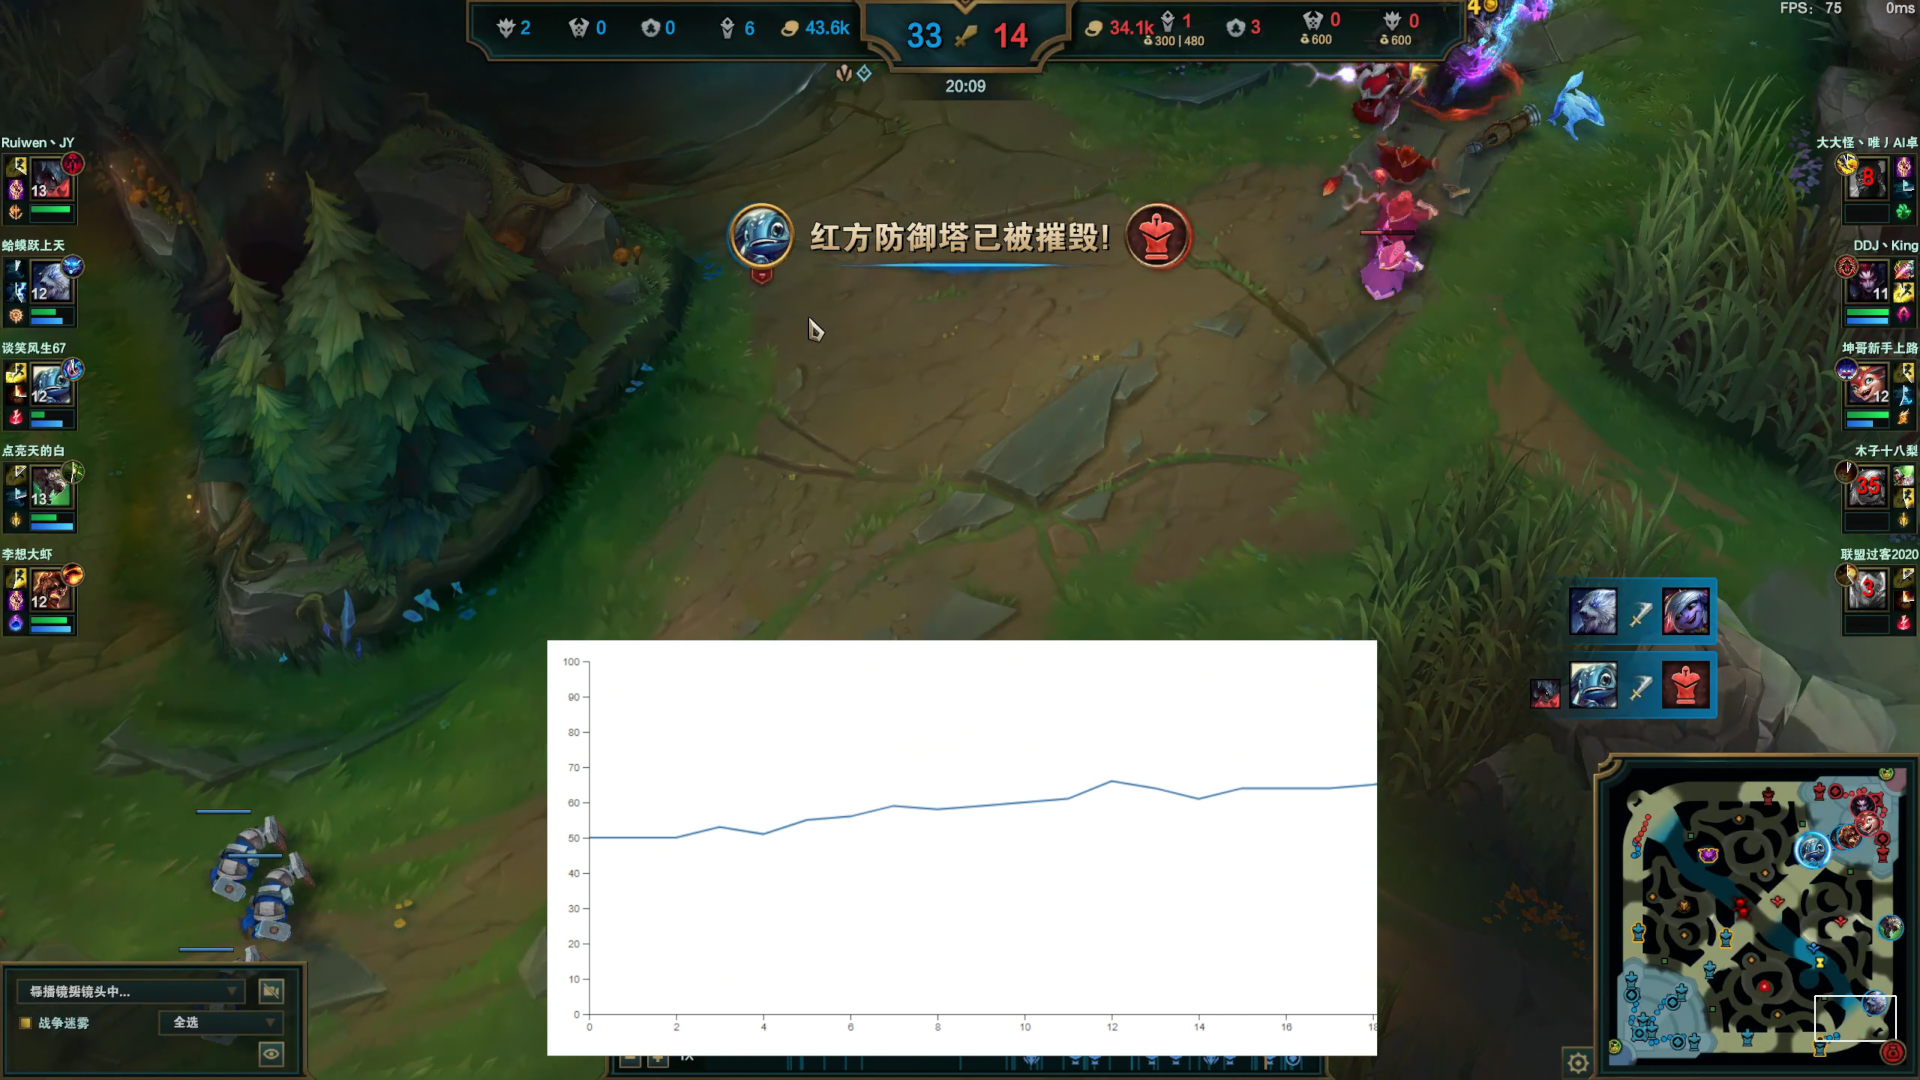
\includegraphics[width=\textwidth]{assets/in_game_pred.png}
  \caption{In-game Prediction Overlay}
  \label{fig:in_game_pred}
\end{figure}

To incorporate the overlay into a live stream, it can be added as a browser source in \href{https://obsproject.com/}{OBS Studio}. This allows the overlay to be displayed on top of the streaming content, similar to the overlays used in professional esports broadcasts.

At its current stage, the overlay may have a simple appearance, as shown in Figure \ref{fig:in_game_pred}. However, there is room for future improvements to enhance its visual appeal. Additionally, additional features can be implemented, such as displaying game events like objective takedowns and champion kills within the line chart as in Figure \ref{fig:edg_vs_wbg_g4_wp} and Figure \ref{fig:t1_vs_wbg_g2_wp}.

%%%%%%%%%%%%%%%%%%%%%%%%%%%%%%%%%%%%%%%%%%%%%%%%%%%%%%%%%%%%%%%%%%%%%%%%%%%%%%%%

\chapter{Discussion}
\label{discussion}

The pre-game prediction model achieves an accuracy of approximately 70\%. On the other hand, the accuracy of the LSTM model for in-game prediction starts around 50\% and gradually improves to nearly 100\% as the game progresses.

It might appear surprising that the in-game LSTM model performs better only after the around 10 minutes, while the pre-game prediction model exhibits higher accuracy before that point as LSTM model captures temporal dependencies and has much more parameters than the logistic regression one. This discrepancy can be attributed to the differences in the input features used by each model. The pre-game prediction model leverages champion mastery and players' past records as input, which provides valuable information about the players' skill and experience. In contrast, the in-game LSTM model does not include these features in its input, and assume each player's skills are the same. Consequently, during the initial stages of the game, where the impact of champion mastery and past records is significant, the pre-game prediction model outperforms the in-game model. However, as the match progresses and more in-game data becomes available, the in-game LSTM model's accuracy increases, capturing the evolving dynamics and performance of the teams.

% As a side note, player often attribute the loss to the Elo rating system when they perform good but their teammates do not.

In the future, we might also include these information about the players' skill and experience in the in-game prediction model to give a more holistic estimation.

Besides, as mentioned in Chapter \ref{sec:embedding}, we could improve our champion-item embedding model by ways like incorporating the influence of runes and adopt negative sampling.

%%%%%%%%%%%%%%%%%%%%%%%%%%%%%%%%%%%%%%%%%%%%%%%%%%%%%%%%%%%%%%%%%%%%%%%%%%%%%%%%

\chapter{Conclusions}
\label{conclusions}

\instructions{This section is written to put the interpretation of the results
  into the context of the original problem.~ Do not repeat the discussion
  points or include irrelevant material. The conclusion should be based on
  the evidence presented.}


The integration of machine learning techniques within the dynamic landscape of League of Legends has demonstrated its immense value in strategic decision-making and accurate predictions. This project has successfully utilized the Riot API, LCU, and machine learning algorithms to develop pre-game and in-game prediction applications.

By gathering data from the Riot API and statistics websites, training machine learning models, and applying word embedding techniques, this project has provided valuable insights into champion and item compatibility. These insights enable players to make informed decisions during gameplay, enhancing their strategic choices.

Moreover, the project has employed LSTM models for real-time in-game win rate prediction. This prediction capability is particularly significant in high-stakes tournaments such as the Worlds and MSI, where accurate in-game predictions can be a useful interpretation of the game

Through the development of machine learning applications using Tauri and React, and backend integration with the League Client, this project has created tools that empower players to improve their performance on the Summoner's Rift. By offering valuable predictions and insights, players can make informed decisions, thereby enhancing their gameplay and overall success in competitive matches. Additionally, the in-game prediction overlay can be utilized in broadcasting LoL matches in spectator mode, adding value to the viewing experience.

Throughout this project, we embarked on an exploration of data acquisition and analysis in League of Legends, delved into various machine learning models, and successfully built applications that leverage these models. The implementation of this project highlights the growing significance of machine learning techniques in the realm of League of Legends, both in the context of esports and daily gameplay. It also showcases the potential for developers to explore and create engaging and valuable applications using the Riot API and LCU API. As the game continues to evolve, the integration of these technologies is expected to become even more prevalent, further enhancing the strategic depth and competitiveness of League of Legends.

%%%%%%%%%%%%%%%%%%%%%%%%%%%%%%%%%%%%%%%%%%%%%%%%%%%%%%%%%%%%%%%%%%%%%%%%%%%%%%%%

\chapter*{References}
\label{references}
\addcontentsline{toc}{chapter}{References}


\instructions{Many bibliographic styles are acceptable for publications
  in the natural sciences. This template uses a numeric style defined in biblatex
  and that is common in Physics, Mathematics, and Computer Science papers.}

\printbibliography[heading=none]

%%%%%%%%%%%%%%%%%%%%%%%%%%%%%%%%%%%%%%%%%%%%%%%%%%%%%%%%%%%%%%%%%%%%%%%%%%%%%%%%

% \appendix

% \chapter{Game Related Information}
% \label{appendix-a}

% As a player on the China server operated by Tencent, I understand the need for English-to-Chinese terminology translations. Below is a lookup table providing translations for various game terminologies. Please note that some terms may not have direct equivalents in Chinese, so the translations provided are the closest approximations.

% \section{English to Chinese Game Terminologies}

% \begin{longtable}{cc}
%   \hline
%   \textbf{English}          & \textbf{Chinese} \\
%   \hline
%   Champion                  & 英雄               \\
%   Minion                    & 小兵               \\
%   Monster                   & 野怪               \\
%   Jungle                    & 野区/打野            \\
%   River                     & 河道               \\
%   Creep Score               & 补刀数              \\
%   Item                      & 装备               \\
%   Gold                      & 金币               \\
%   Structure                 & 建筑物              \\
%   Turret                    & 防御塔              \\
%   inhibitor                 & 召唤水晶             \\
%   Nexus                     & 水晶枢纽             \\
%   Rift Herald               & 峡谷先锋             \\
%   Baron Nashor              & 纳什男爵             \\
%   Voidmite                  & 虚空潮虫             \\
%   ARAM (All Random All Mid) & 极地大乱斗            \\
%   Summoner's Rift           & 召唤师峡谷            \\
%   lanes                     & 兵线               \\
%   Ranked                    & 排位               \\
%   Normal                    & 匹配               \\
%   Farming                   & 发育               \\
%   Experience                & 经验值              \\
%   Controller                & 控制者,控场者          \\
%   Enchanter                 & 附魔者,软辅           \\
%   Catcher                   & 捕手,利用点控单点突破      \\
%   Fighter                   & 战士               \\
%   Juggernaut                & 重装战士             \\
%   Diver                     & 轻装战士             \\
%   Mage                      & 法师               \\
%   Burst                     & 爆发法师             \\
%   Battlemage                & 战斗法师,冲阵法师        \\
%   Artillery                 & 炮台               \\
%   Marksman                  & 射手               \\
%   Slayer                    & 屠宰者,杀手           \\
%   Assassin                  & 刺客               \\
%   Skirmisher                & 游击者              \\
%   Tank                      & 坦克               \\
%   Vanguard                  & 前锋,进攻坦克          \\
%   Warden                    & 后卫,防守坦克          \\
%   Specialist                & 机制特殊类英雄          \\
%   Champion Mastery          & 英雄成就             \\
%   KDA                       & 战损比              \\
%   \caption{English to Chinese Game Terminologies}
%   \label{tab:trans}
% \end{longtable}

% \section{Full List of Champion Attributes}

% \begin{itemize}
%   \item {
%         \textbf{Controller}: Controllers assist their allies with potent utility and keep enemies at bay with crowd control. Weak when alone, supports are capable of massively amplifying their teammates' power to become the strongest class in group combat (or teamfights), supplying crucial utility or crowd control at clutch moments to save allies from death and enable takedowns on the enemy team. Supports typically start out by assisting the marksman in lane, as their own power is less dependent on items to function well, but over time their contribution expands as they lend aid to their entire team with both their spells and effective, yet affordable, items.
%         \begin{itemize}
%           \item \textbf{Catcher}: Catchers specialize in locking down opponents or, in some cases, entire battlefields by creating intense zones of threat that only foolish enemies would dare wade through.
%           \item \textbf{Enchanter}: Enchanters focus on amplifying their allies' effectiveness by directly augmenting them and defending them from incoming threats. Enchanters themselves are often quite fragile and bring relatively low damage to the table, meaning they really only shine when grouped together with others.
%         \end{itemize}
%         }
%   \item {
%         \textbf{Fighter}: Fighters (also known as Bruisers) are a diverse group of short-ranged combatants who excel at both dealing and surviving damage. With easy access to heavy, continuous damage (or DPS) and a host of innate defenses, fighters thrive in extended fights as they seek out enemies to take down, but their limited range puts them at constant risk of being kept at bay (or kited) by their opponents via crowd control, range and mobility.
%         \begin{itemize}
%           \item \textbf{Diver}: Divers are the more mobile yet less durable portion of the Fighter class. Divers excel at singling out high-priority targets to blitz toward, immediately forcing those targets (and their teammates) to deal with the diver's presence.
%           \item \textbf{Juggernaut}: Juggernauts are melee titans who relentlessly march down the opposition and devastate those foolish enough to get within their grasp. They are the only subclass who excel at both dealing and taking significant amounts of damage, but in turn they have a tough time closing in on targets due to their low range and extremely limited mobility.
%         \end{itemize}
%         }
%   \item {
%         \textbf{Mage}: Mages are champions who typically possess great reach, ability-based area of effect damage and crowd control, and who use all of these strengths in tandem with each other to trap and destroy enemies from a distance. Specializing in magic damage, often burst damage, and therefore investing heavily in items that allow them to cast stronger and faster spells, mages excel at chaining their abilities together in powerful combos in order to win fights, though their abilities also tend to be difficult to land and can be mitigated, if not avoided completely, by their targets if they react in time.
%         \begin{itemize}
%           \item \textbf{Artillery}: Artillery Mages are the masters of range, and they leverage that advantage to whittle down their opponents over time from great distances. In turn, Artillery Mages are severely punished when enemies finally succeed in closing in on them, due to their extreme fragility and limited mobility.
%           \item \textbf{Battlemage}: Battlemages (also known as Warlocks) get into the middle of the fray, seeking to wreak havoc upon the entire enemy team with their overwhelming sustained area damage. Due to their relatively short (but not melee) combat ranges and the need to burn down their opponents over time, Battle Mages have significant defensive capabilities that range from sustaining endlessly to literally defying death for a short period of time.
%           \item \textbf{Burst}: Burst Mages aim to single out vulnerable targets by locking them down and following up with a devastating barrage of damage from range. They are strongest when using their full suite of spells executed perfectly to maximum effect, and most vulnerable when they cannot deliver.
%         \end{itemize}
%         }
%   \item {
%         \textbf{Marksman}: Marksmen are ranged champions whose power almost exclusively revolves around their basic attacks: using their reach to land massive continuous damage from a distance, marksmen are capable of taking down even the toughest of opponents when positioned behind the safety of their team. Marksmen are tremendously vulnerable to burst damage, due to their fragility, and tend to be exceptionally weak early in the game, requiring high amounts of gold, mostly via minion kills (or CS: Creep Score) to acquire powerful, but expensive, damage-focused items.
%         }
%   \item {
%         \textbf{Slayer}: Slayers are highly mobile champions who specialize in single target burst damage. What they generally lack in resilience, they more than make up for with their ability to quickly cover large distances, kill priority targets and retreat just as fast. Epitomizing a high risk, high reward playstyle, assassins are natural opportunists and prefer to strike when their targets are alone and vulnerable, rather than engage them in a direct assault, favoring damage-oriented item builds to capitalize on their offensive capabilities. They're particularly effective against softer (or squishy) targets, especially mages and marksmen, but often struggle against the heightened defenses of fighters and tanks.
%         \begin{itemize}
%           \item \textbf{Assassin}: Assassins specialize in infiltrating enemy lines with their unrivaled mobility to quickly dispatch high-priority targets. Due to their mostly melee nature, Assassins must put themselves into dangerous positions in order to execute their targets. Luckily, they often have defensive tricks up their sleeves that, if used cleverly, allow them to effectively avoid incoming damage.
%           \item \textbf{Skirmisher}: Skirmishers (also known as Duelists) aim to shred through any nearby enemy that approaches. Because Skirmishers lack high-end burst damage or reliable ways of closing in on high-priority targets, they are instead armed with situationally powerful defensive tools to survive in the fray, along with extreme sustained damage to cut down even the most durable targets.
%         \end{itemize}
%         }
%   \item {
%         \textbf{Specialist}: Specialists are a diverse group of champions who do not ``fit into a neat little box'' in regards to other class/subclass specifications.
%         }
%   \item {
%         \textbf{Tank}: Tanks are tough melee champions who sacrifice damage in exchange for powerful crowd control. While able to engage enemies in combat, a tank's purpose isn't usually to kill opponents; rather, tanks excel at disrupting enemies and diverting focus to themselves, allowing them to lock down specific targets (or several targets at once), as well as remove (or peel) threats from their allies.
%         \begin{itemize}
%           \item \textbf{Vanguard}: Vanguards are offensive tanks. Vanguards lead the charge for their team and specialize at bringing the action. Their explosive team fight initiation seeks to catch enemies out of position while allowing allies to follow-up to devastating effect.
%           \item \textbf{Warden}: Wardens are defensive tanks. Wardens stand steadfast, seeking to hold the line by persistently locking down any on-comers who try to pass them. Wardens keep their allies out of harm's way and allow them to safely deal with enemies caught in the fray.
%         \end{itemize}
%         }
% \end{itemize}

% \chapter{Project Setup}
% \label{appendix-b}

% %This template can be viewed on Overleaf at \url{https://www.overleaf.com/read/hxjcgtkhjqcd}.
% % If you have an Overleaf account (either free or paid) you can copy this template to start a new Overleaf project.
% % If you do not want an Overleaf account you can install TeX on your computer and download the template files from Sakai.

% This section is focused on the development aspect and serves as a README of the project, so it is included in the appendix.

% \section{Pre-game Prediction Application with Tauri}

% The Pre-game Prediction Application is developed for Microsoft Windows. While there is a macOS version of League of Legends for the global server, our application has not been tested on that platform. Therefore, the Tauri application is built and tested on Windows.

% Tauri utilizes the Webview component specific to each platform, and it is recommended to ensure that your system is up to date to maintain consistent behavior. Windows 11 or the latest version of Windows 10 should work fine.

% Tauri is built with Rust, so before proceeding, you need to have the Rust toolchains installed on your PC.

% To install Rust, you will first need to install the MSVC build tools. Once the MSVC build tools are installed, you can proceed to install rustup, which is a command-line tool for managing Rust versions and associated tools. For detailed instructions, you can refer to the official installation guide provided by Rust: \href{https://doc.rust-lang.org/book/ch01-01-installation.html}{Rust Installation Guide}.

% Following the installation guide from Tauri (\href{https://tauri.app/v1/guides/getting-started/prerequisites}{Tauri Installation Guide}), you will also need to install Node.js and tauri-cli.

% After installing all the necessary toolchains, you can navigate to the root directory of the Tauri application and run the following commands:

% \begin{verbatim}
% cd tauri
% cargo tauri dev # or cargo tauri build for production
% \end{verbatim}

% This will launch the Tauri application, and you should now be able to use it accordingly.

% \section{In-game Prediction Machine Learning Backend with Flask}

% \section{In-game Prediction Frontend with React}

\end{document}
